TODO: rewrite
\begin{itemize}
	\item mention TS-ADC paper from the 90s (technique is already known since then, a lot of development )
	\item briefly explain the evolution over the past 20/30 years
	\item transition to usage of TS in physics
\end{itemize}

Observing non-repetitive and statistically rare signals that occur on short timescales requires fast real-time measurements that exceed the speed, precision and record length of conventional digitizers. Photonic time stretch is a data acquisition method that overcomes the speed limitations of electronic digitizers and enables continuous ultrafast single-shot spectroscopy, imaging, reflectometry, terahertz and other measurements at refresh rates reaching billions of frames per second with non-stop recording spanning trillions of consecutive frames. The technology has opened a new frontier in measurement science unveiling transient phenomena in nonlinear dynamics such as optical rogue waves and soliton molecules, and in relativistic electron bunching. It has also created a new class of instruments that have been integrated with artificial intelligence for sensing and biomedical diagnostics. We review the fundamental principles and applications of this emerging field for continuous phase and amplitude characterization at extremely high repetition rates via time-stretch spectral interferometry.

A new generation of instruments based on photonic time stretch is opening the path to measuring and understanding the behaviour of non-stationary and rare phenomena in ultrafast systems, and harvesting their potential for practical applications such as metrology, machine vision and biomedicine. While these instruments rely on optics for the transformation of a signal's timescale, they are able to operate with either electrical, optical, or terahertz inputs. \cite{szwaj}




\section{Time-Stretching Techniques in Physics}
\begin{itemize}
	\item Relativistic electron beam diagnostics
	\item Characterization of noise and fluctuations in nonlinear optics
	\item Laser dynamics
\end{itemize}


\section{Motivation}
When doing science with terahertz radiation and in some laser applications, ultrafast events need to be characterized.
Commercially available real-time equipment is limited in bandwidth (240 GS/s, LeCroy LabMaster 10-100Zi) and cannot be used to characterize these events in the pico- and femto-second regime.
In this thesis you will evaluate a real-time measurement technique based on the photonic time-stretch analog-to-digital converter (TS-ADC) for the measurement of ultrafast signals with a sampling-rate which exceeds TS/s.
The principle is to use a photonic front-end that effectively ``slows down'' the analog signal in time before it is digitized by fast \glspl{adc}.

\begin{figure}[tbh]
	\centering
	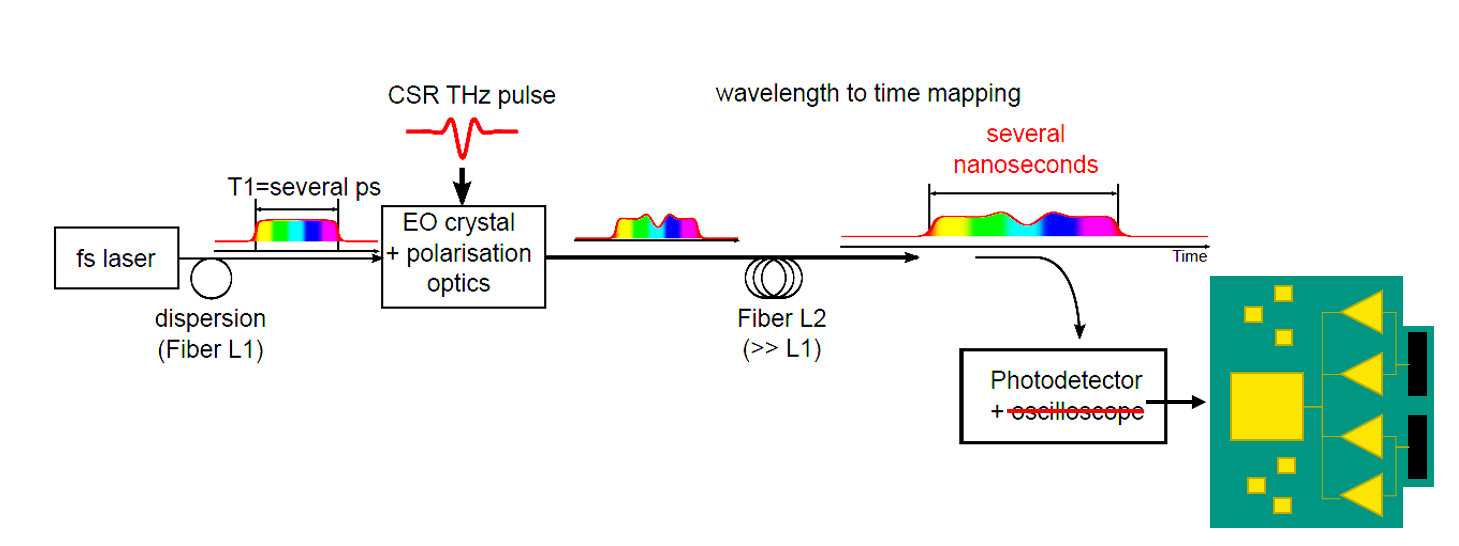
\includegraphics[width=\textwidth]{chap/02-theory/img/motivation}
	\caption{Use case of the system}
	\label{fig:motivation}
\end{figure}
%todo to tikz

\subsection{THz Science and Coherent Synchrotron Radiation}
\textbf{TODO:} Explain physical expressions

\Gls{sr} is produced in synchrotron radiation facilities (like electron storage rings) by accelerating relativistic electrons.
Emission of \gls{sr} occurs, when electron beams are bent or deflected with dipole magnets or using an undulator\footnote{Undulators are used to make the electrons oscillate by generating a periodic magnetic field}. 

\autoref{fig:storageRing} shows the general scheme of an electron storage ring.
Electrons, or rather electron bunches, are generated with an electron gun and are accelerated to almost the speed of light by a \gls{linac}.
After being broad up to their nominal energy in a booster, the bunches are then injected into the storage ring.
In the ring, the path of the electron bunches is altered by bending magnets, guiding them on a circular trajectory.
Due to emission of \gls{sr} at each bend, the electrons lose energy, which has to be compensated for.
This is done by accelerating them with an electric field inside a \gls{rf} cavity.
Not shown in the drawing are the beamlines, which lead the \gls{sr} radiation, or rather chosen wavelength ranges, through an optical system to the respective user experiments. \cite{roussel2014} \cite{rota2018}

\begin{figure}[tbh]
	\centering
	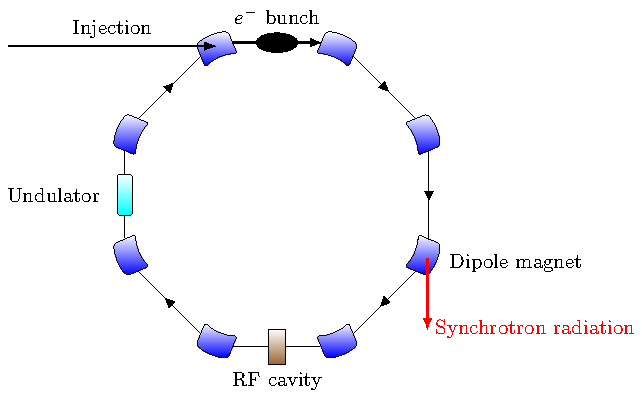
\includegraphics[width=0.7\textwidth]{chap/02-theory/img/synchrotron}
	\caption{Basic scheme of an electron storage ring (redrawn from \cite{roussel2014})}
	\label{fig:storageRing}
\end{figure}
%todo where's the booster?
\paragraph{Karlsruhe Research Accelerator}
\textbf{TODO:} Brief overview over \gls{kara}
\begin{itemize}[noitemsep]
	\item Located at the Karlsruhe Institute of Technology (KIT)
	\item Up to 184 electron bunches can be filled into the storage ring with a distance of \SI{2}{\nano\second} (\SI{500}{\mega\hertz}) between two adjacent bunches
	\item Operated by the Institute of Beam Physics and Technology (IBPT)
	\item Microtron, Booster Synchrotron, and Storage Ring
\end{itemize}

\begin{table}[tbh]
	\caption{Some KARA parameters \cite{rota2018}}
	\label{tab:kara}
	\centering
	\begin{tabular}{ll}
		\toprule
		\textbf{Parameter}                  & \textbf{Value}                \\ \midrule
		Beam energy                         & \SI{2.5}{\giga \electronvolt} \\
		Circumference                       & \SI{110}{\meter}              \\
		Revolution Frequency (one electron) & \SI{2.7}{\mega \hertz}        \\
		             \multicolumn{2}{c}{Minimum bunch spacing}              \\
		\quad multi-bunch                   & \SI{2}{\nano \second}         \\
		\quad single-bunch                  & \SI{368}{\nano \second}       \\
		                 \multicolumn{2}{c}{Bunch length}                   \\
		\quad normal operation              & \SI{45}{\pico \second}        \\
		\quad short bunch                   & \SI{2}{\pico \second}         \\ \bottomrule
	\end{tabular}
\end{table}

The range of \gls{sr} reaches from hard X-rays down to the infrared region of the electromagnetic spectrum (see \autoref{fig:spectrum}). In contrast to other sources, it has properties like:
%todo which sources, convert list to text?
\begin{itemize}[noitemsep]
	\item high intensity 
	\item high collimation
	\item polarisation
	\item well-defined timing of pulses
\end{itemize}

Due to this properties, synchrotrons are used for microscopy, spectroscopy, and time-resolved experiments in such fields like condensed matter physics, biology, material science and many more.
%todo why are these imporant for the applications listed here. maybe pick one and explain it in more detail and/or an equation
\begin{figure}[H]
	\centering
	\includegraphics[width = \textwidth, height = 0.5\textwidth]{chap/02-theory/img/spectrum.tikz}
	\caption{Electromagnetic spectrum} %todo of what?
	\label{fig:spectrum}
\end{figure}
%todo 7 column not working for some reason, 
%todo replace with measured I(\lambda)/I_0 plot?
%todo unit (\si{\micro\meter}) instead of []

\subsubsection*{Micro-Bunching Instabilities}
Increasing demands in current and future accelerators call for higher brilliance of the emitted radiation.
%todo define brilliance, flux, emittance
This is achieved by increased photon flux and reduction of the transverse emittance.
For longitudinal coherence, the electron bunches are shortened, which results in emission of \gls{csr} at frequencies up to the THz range.
%todo how does coherence relate to the terms mentioned earlier?

However, this introduces complex dynamics, as the electrons interact with their own radiation.
This manifests into the so called micro-bunching instability.
The formation of micro-structures (in the sub-millimeter to centimeter range) in the longitudinal density profile of the electron bunches.
Being on the one side a limitation to the stable operation of the overall system at high current density/short bunch length mode.
On the other side, these instabilities can be potential sources of brilliant THz radiation. %todo why
A thorough understanding of these dynamics is necessary to control the emission in this spectral domain which enables usage in experiments. \cite{rota2018,brosi}

\begin{figure}[tbh]
	\centering
	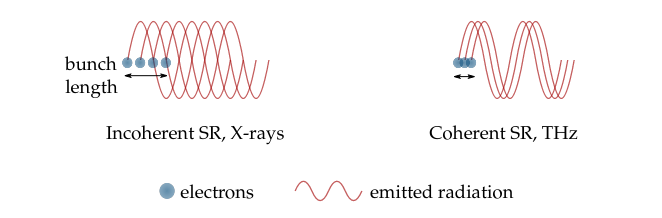
\includegraphics[width = \textwidth]{chap/02-theory/img/csr2.png}
	\caption{Incoherent \gls{sr} and coherent \gls{sr} due to shorter electron bunch length \cite{rota2018}}
	\label{fig:csr}
\end{figure}
%todo to tikz

\begin{figure}[tbh]
	\centering
	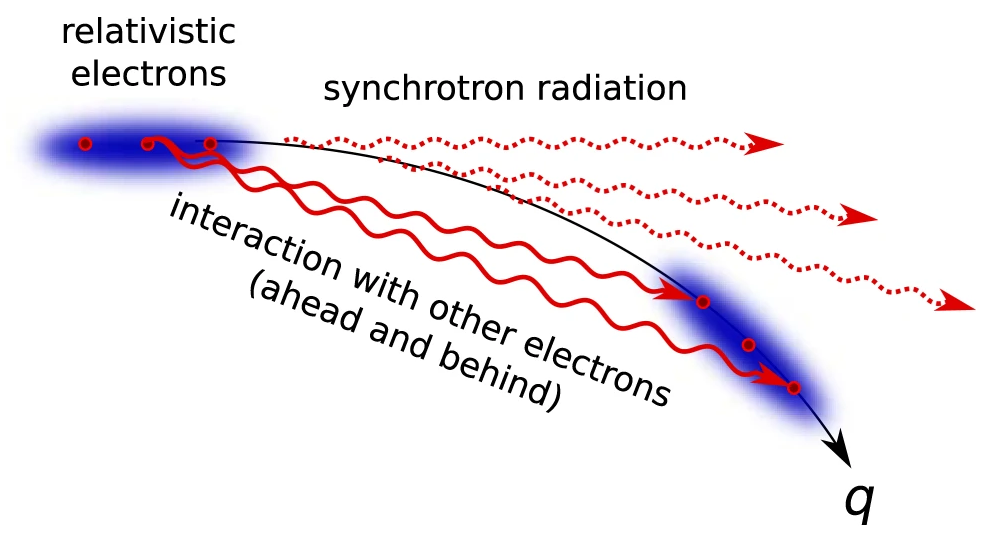
\includegraphics[width = 0.5\textwidth]{chap/02-theory/img/microbunching}
	\caption{Electrons interact with their own radiation \cite{Bielawski2019}}
	\label{fig:microBunch}
\end{figure}


\subsection{Longitudinal Bunch Profile Diagnostics}

\subsubsection*{Scanning-Type Electro-Optic Sampling}
The 
%todo what is that, one sentence
A short laser pulse (duration typically hundreds of femtoseconds) co-propagates with a THz pulse from \gls{csr} (range of picoseconds) in an \gls{eo} crystal. Due to the Pockels effect\footnote{"The Pockels effect denotes the occurrence of
	and change in existing birefringence in an electric field linearly, which is proportional to the electric
	field strength. \cite{pockels}} the THz pulse causes a time dependent birefringence in the crystal.
%todo avoid direct quote
This modulates the polarization of the laser pulse.
To sample the pulse, the delay between the laser and the THz pulse is varied.
To detect the changing polarization, the polarization of the laser pulse is transformed into an intensity modulation.
A general scheme of the system is shown in \autoref{fig:scan_eo}.
For this technique a stable emission of the THz pulses is crucial, as they are not measured in one acquisition. \cite{roussel2014}
\begin{figure}[tbh]
	\centering
	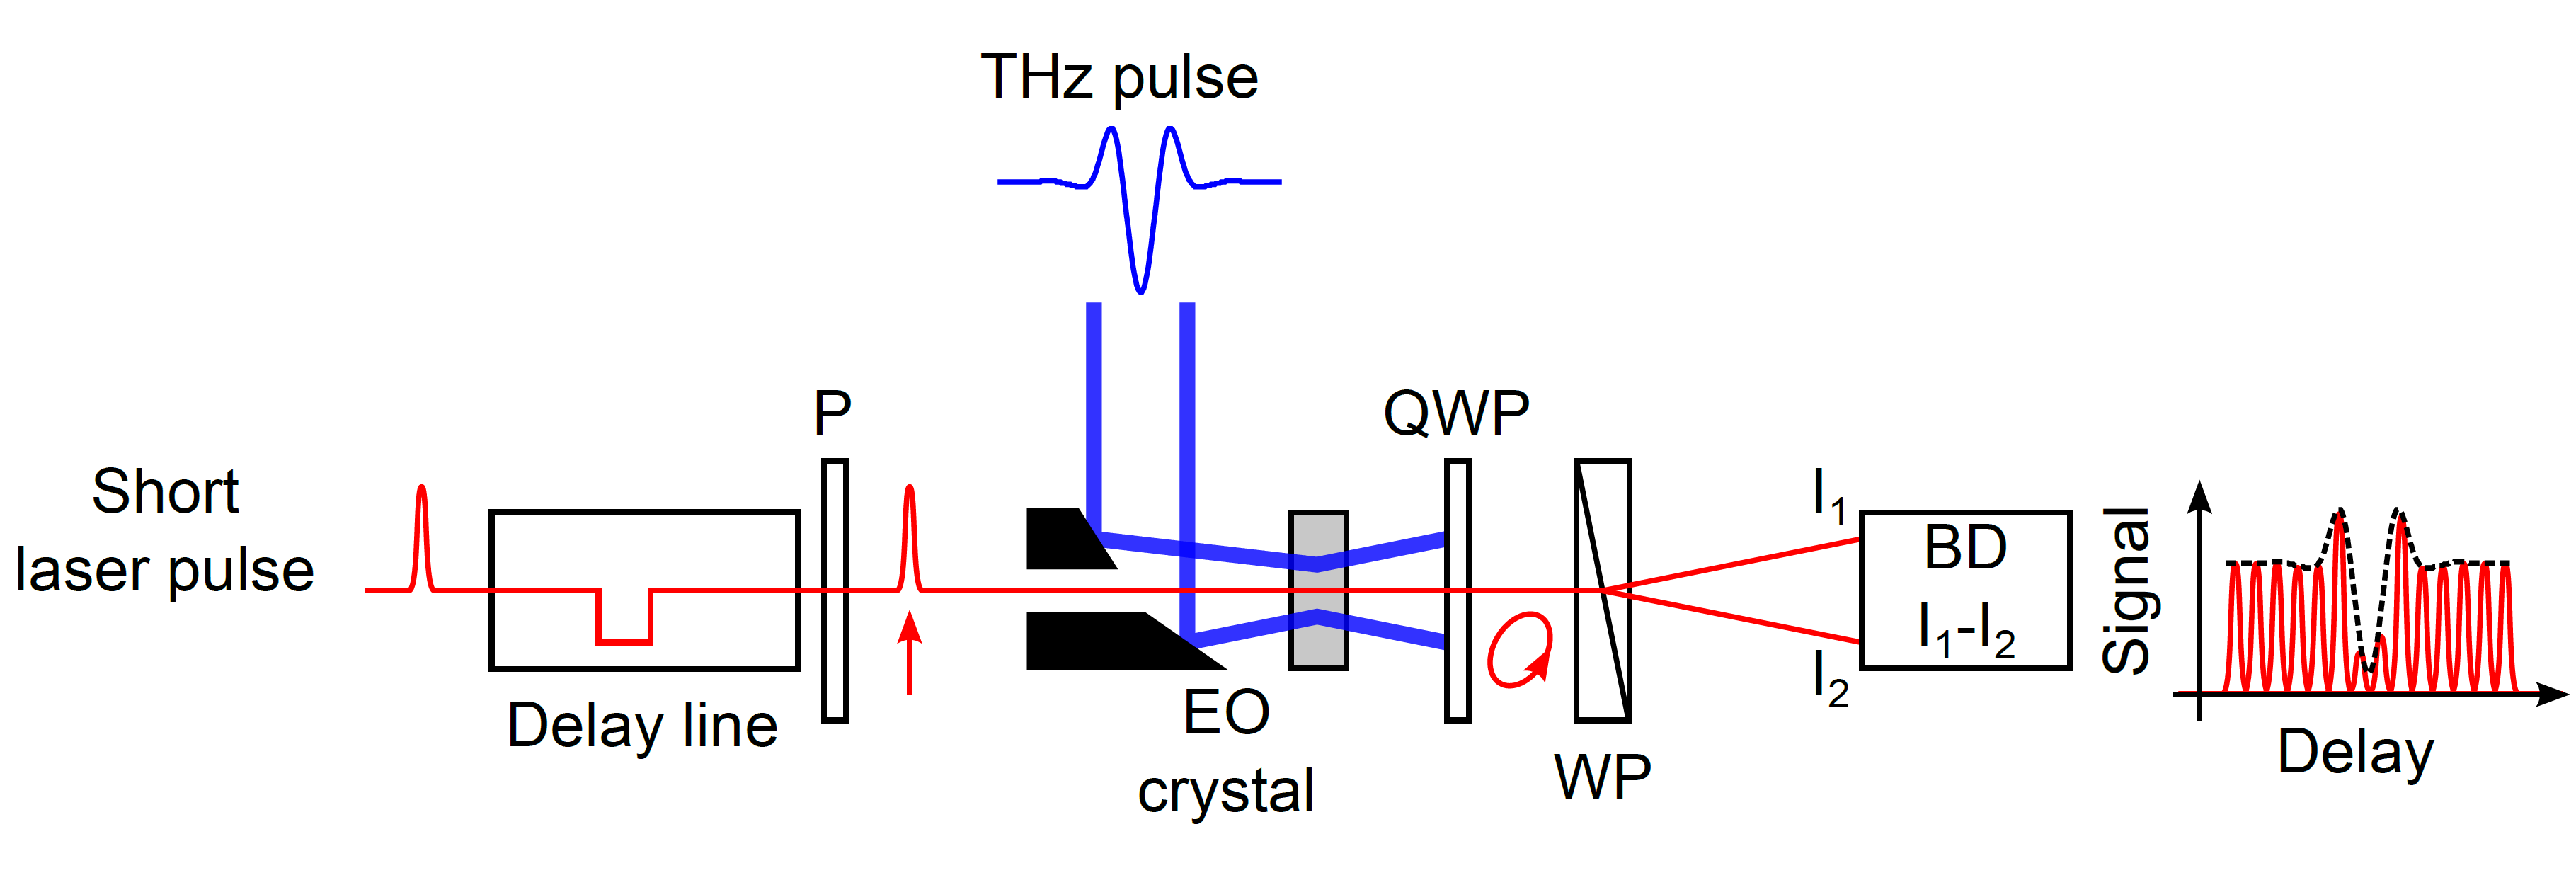
\includegraphics[width = 0.8\textwidth]{chap/02-theory/img/scanning_eo}
	\caption{Scheme of Scanning-Type Electro-Optical Sampling System \cite{roussel2014}}
	\label{fig:scan_eo}
\end{figure}

\subsubsection*{Spectrally Resolved Electro-Optic Detection}
In contrast to the EOS, single-acquisition is possible with the spectrally resolved electro-optic detection technique. %todo EOS==EO?
The short laser pulse is first stretched to a duration similar to the Thz pulse in a dispersive material (stretcher).
In this way the pulse is chirped, meaning the instantaneous frequency of the pulse varies over time.
Together with the THz, the laser pulse propagates in a \gls{eo} crystal.
Again, the induced birefringence modulates the laser pulse, not only in time, but also in the optical spectrum.
The polarization state of the pulse is converted into an amplitude/intensity modulation.
To retrieve the THz pulse shape in time, the spectrum of the laser pulse is measured with a spectrometer. %todo what spectrometer (optical or electrical) or state model
A general scheme of the system is shown in \autoref{fig:spectral_eo}. \cite{roussel2014}

\begin{figure}[tbh]
	\centering
	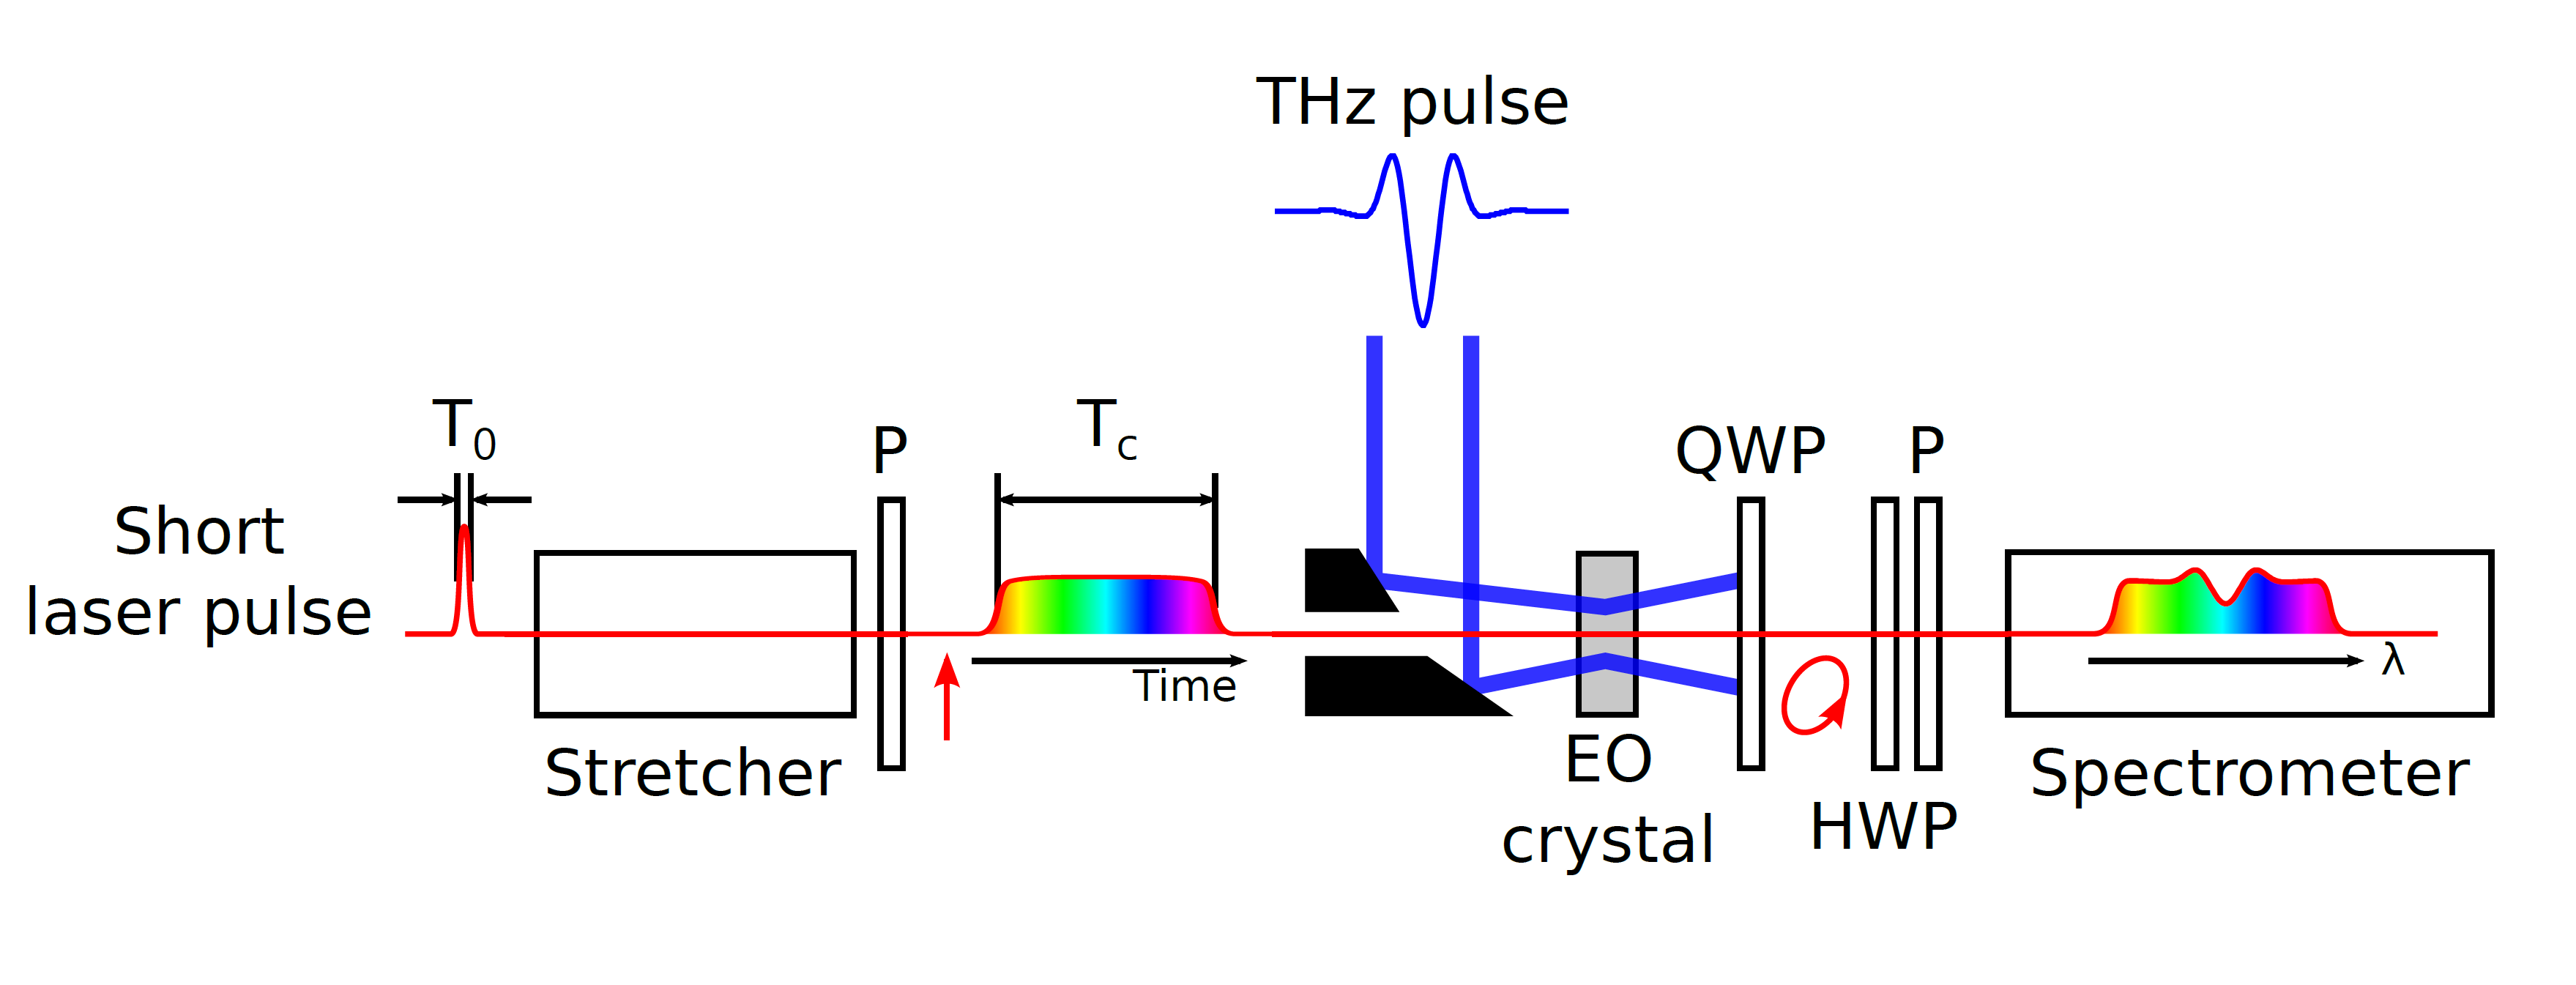
\includegraphics[width = 0.8\textwidth]{chap/02-theory/img/spectral_eo}
	\caption{Scheme of Spactrally Encoded Electro-Optical Detection System \cite{roussel2014}}
	\label{fig:spectral_eo}
\end{figure}

The temporal resolution of this method is limited due to the finite chirp rate
\begin{equation}
	\text{chirp rate} = \frac{\text{laser bandwidth}}{\text{laser pulse duration after stretcher}}.
\end{equation}

The resolution $T_{\text{min}}$ is determined as
\begin{equation}
	T_{\text{min}} = \sqrt{T_0 T_c}
\end{equation}
with the bandwidth-limited pulse duration (before stretcher) $T_0$ and the duration of the chirped laser pulse $T_c$.


\textbf{TODO}: refer also to KALYPSO


\subsection{Potential Usage: ANR-DFG ULTRASYNC project?}
From Serge's email:

For accelerator applications, we have also a project (ANR-DFG ULTRASYNC project) with KARA and SOLEIL.
There is the question of control (i.e., suppression) of the bursts occuring during the microbunching instability. The objective is to obtain a high power and stable coherent emission (at SOLEIL and KARA). For the moment, the only experimental test has been made using a relatively simple feedback:
\begin{itemize}
	\item a bolometer signal as the feedback loop input
	\item a low-cost FPGA (redpitaya) that sends the feedback on the accelerating voltage
\end{itemize}

There are limitations in the maximal bunch charge in the accelerator. So an open question is whether measuring each THz pulse using EO sampling + time-stretch may help to solve this open problem. In clear:

\begin{itemize}
	\item EO sampling + time-stretch as in Eléonore's thesis
	\item association with the new FPGA-based system
	\item finding adequate feedback that is programmed in the FPGA
\end{itemize}
may solve the problem, and allow the control to succeed at the highest currents in SOLEIL. 
Target would be ca. 15 mA for 1 bunch (and feedback control presently works to a little more than ca. 10 mA).

\section{Objective}
Design of a system to be used with photonics time-stretch technique. Fast, continuous sampling of signals, integratable in already existing high data-throughput architectures.






%\begin{itemize}
%	\item Microbunching instabilites $\rightarrow$ THz radiation $\rightarrow$ Potential source of brilliant radiation
%	\item Need to be studied to be able to control it
%	\item Time-resolution critical, as instabilities have high bandwidth
%	\item Commercial oscilloscopes don't have enough internal memory
%	\item already developed system KAPTURE/KAPTURE-2 to solve this problem
%	\item however: four/eight points not enough to see the microbunching instabilities
%	\item Concept: combine time-stretch with FPGA $\rightarrow$ THERESA (\textbf{T}era\textbf{He}rtz \textbf{Re}adout \textbf{Sa}mpling)
%	\item EO technique to stretch the signal in time, so requirements on the bandwidth of converters can be relaxed
%	\item more converters, to have more points
%	\item New generation FPGA/SoC for fast readout and high data throughput
%\end{itemize}
%
%Available commercial DAQ system or real-time oscilloscopes for high bandwidth (e.g. above
%40 GHz) are very expensive and, due to limited internal memory and missing fast readout interfaces, are not suitable for long term bunch-to-bunch CSR measurements. To circumvent these limitations a DAQ architecture for fast and continuous sampling of the individual ultra-short THz pulses has been developed.









%
%
%
%
%The past decade has seen the rapid development of CSR studies in many storage
%rings. Despite the large amount of experimental observations, e.g. the recordings
%of coherent THz bursts, lack of direct observation of the electron bunch and its
%microstructures is a main issue to the test and development of the theoretical models.
%Even though in chapter 5 we presented first real-time measurements of CSR
%pulses using a YBCO superconductor-based detector at UVSOR-III, a majority
%of storage rings emits coherent synchrotron radiation at higher frequencies than
%the state-of-the-art oscilloscope bandwidth (currently 65 GHz), e.g. 300 GHz
%at SOLEIL [8],250 GHz at ANKA [2],500 GHz at ELETTRA [5].
%
%Spontaneous formation of small-scale microstructures can have a deleterious effect on electron bunch stability and emission properties, and they are at the same time a tremendous source of coherent radiation in the terahertz domain3,4,5,6,7,8,9,10,11,12,13,14,15,16,17, provided the instability can be mastered. This is the reason why understanding and controlling the interplay between Coherent Synchrotron Radiation (CSR) and the microbunching instability has nowadays become a central open question in the development of synchrotron radiation facilities.
%
%To answer this question, it is essential to develop ultrafast photonic devices for electron bunch shape characterization. The challenges for the photonics community is high, given the need for ultrashort (picosecond or femtosecond) temporal resolution, single-shot operation, at high repetition rates (MHz and more), and given the particularly challenging environment near relativistic electron bunches. Recent advances consequently pushed photonics systems beyond the state of the art. Ultrafast electric-field measurement techniques using femtosecond laser pulses (electro-optic sampling24) have allowed single-shot bunch shape measurements (plural)25, and these techniques have then been extensively investigated and improved this last decade
%
%
%The ULTRASYNC (Exploration et contrôle ULTRArapide de la dynamique des paquets d'électrons dans les sources de lumière SYNChrotron, ANG-DFG) aims to study and control coherent synchrotron radiation (CSR) and microbunching instability. The goal is to obtain a high power and stable coherent emission (KARA and SOLEIL) by feedback control. At SOLEIL, this was already succesfully achieved, still there is a significant limit to the range, where this concept works. One possible way would be to calculate the necessary feedback from a whole THz CSR pulse shape, which would require to record an electro-optical signal (time-stretch). This leads to a possible approach by combining time-stretch and FPGA. 
%
%For the moment, the only experimental test has been made using a relatively simple feedback:
%- a bolometer signal as the feedback loop input
%- a low-cost FPGA (redpitaya) that sends the feedback on the accelerating voltage
%There are limitations in the maximal bunch charge in the accelerator. So an open question is whether measuring each THz pulse using EO sampling + time-stretch may help to solve this open problem. In clear:
%- EO sampling + time-stretch as in Eléonore's thesis
%-> association with the new FPGA-based system
%-> finding adequate feedback that is programmed in the FPGA
%may solve the problem, and allow the control to succeed at the highest currents in SOLEIL. 
%Target would be ~15 mA for 1 bunch (and feedback control presently works to a little more than ~10 mA).
%
%At 1 micron wavelength, the maximum stretch is limited due to fiber glass properties (at this wavelength). The maximum length achieved are 2-4 ns (SOLEIL and KARA). For this reason, a fast ADC is critical, to get a good ENOB/number of sampling points. A relevant figure of merit (that characterizes the effective number of points) is -- we think: FOM=electronic bandwidth x stretch time. There is some bottleneck concerning time-stretch at this wavelength, and one way to solve the issue is to try pushing the bandwidth of ADCs.
%
%At 1550 nm wavelength, it is possible to stretch the signal up to tens of nanoseconds. Therefore, a relatively cheap ADC would already be sufficient and allow an effective number of samples at around 100. Applications still need to be investigated.
%
%As potential applications for the new system would be applications for accelerators in the 1 micron wavelength (best concerning EO sampling SNR and bandwidth).
%
\section{General Architecture of a Photonic Time-Stretch Data Acquisition System}
In this section, a general architecture of a Photonic Time-Stretch \gls{daq} is described.
Such a system consists of a photonic front-end, which covers the time-stretching method and conversion of photons into electrical values. %todo system= front-end? or front-end + ...?
In the following, the general theory of the time-stretching technique is given together with some photo-detector fundamentals. 

%todo rewrite from ...
Furthermore, such a system contains an \gls{adc} which converts the analog values into digital signals that can be processed by a computing unit. A short overview of the basic \gls{adc}-theory is given, as well as of the most prominent figures of merit. Knowledge and understanding of these is necessary to define and/or evaluate the overall performance of the converter. 

Last but not least a \gls{daq} needs an appropriate computing system for collection, processing and visualization of the acquired data. As this part is use-case specific, there doesn't exist a general "theory" which can be described.
%todo to here

\subsection{Photonic Time-Stretch Front-End}
The working principle of the optic time-stretch technique can be described in two steps (see \autoref{fig:eo_ts}).

First, a short laser pulse (duration typically hundreds of femtoseconds) propagates in a dispersive medium, e.g. an optical fiber of length $L_1$ (see \autoref{fig:eo_ts}).
This results in a chirped laser pulse of the duration
\begin{equation}
	T_1 = \Delta \lambda D_1 L_1
\end{equation}
with the optical bandwidth of the laser pulse $\Delta \lambda$  and the dispersion parameter $D_1$ of the fiber.

%todo is this the second step?
The next step is the time-to-wavelength-mapping, where a temporal intensity modulation is imprinted on the chirped pulse.
In this step, the laser pulse co-propagates with another pulse, e.g. a \gls{thz} pulse from \gls{csr} (duration in the range of picoseconds), in an \gls{eo} crystal. Due to the Pockels effect\footnote{The Pockels effect describes the phenomenon of occurring and change of existing birefringence in an electric field, which is linearly proportional to the electric field strength." \cite{pockels}} the \gls{thz} pulse causes a time-dependent birefringence in the crystal.
This modulates the polarization of the laser pulse.

%todo is this the second step?
After that, the modulated chirped pulse propagates through another dispersive medium, a fiber of the length $L_2$.
In this way, the temporal modulation of the pulse is further stretched to the duration $T_2$, which is long enough for detection with photodetectors and the digitizing with \Glspl{adc}. \cite{roussel2014}

The factor, by which the pulse is slowed down, is calculated as
\begin{equation}
	M = 1 + \frac{L_1}{L_2}.
\end{equation}
%todo how does that fit in the explenation above? maybe state some numbers here (<<now by using eq 123, the pulse is xyz long which a fast adc can detect>> or sth like that)

\begin{figure}[tbh]
	\centering
	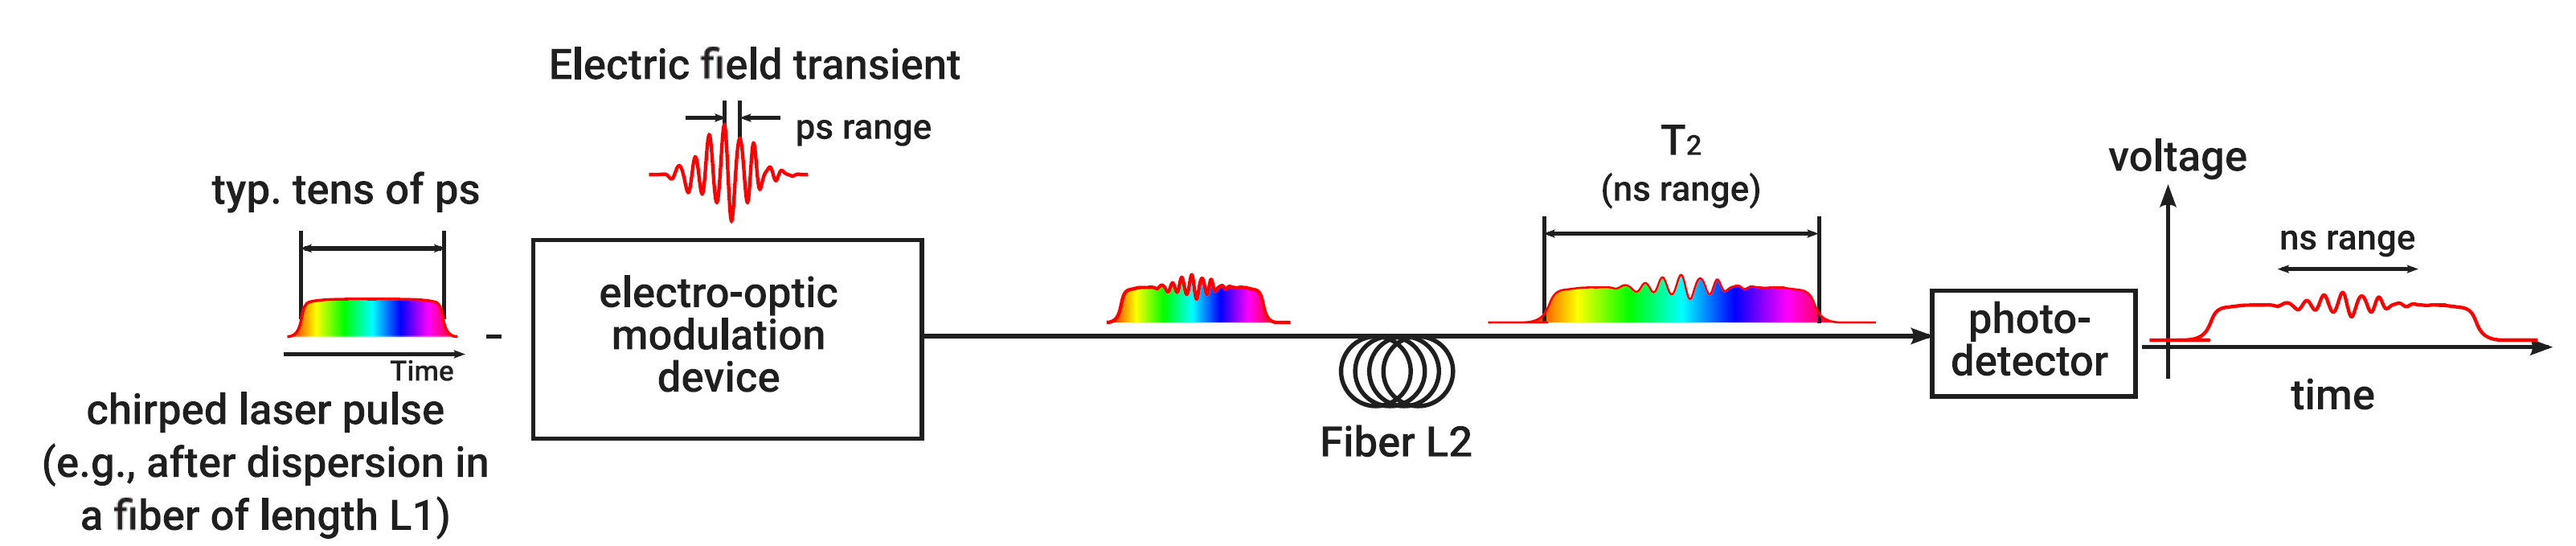
\includegraphics[width = \textwidth]{chap/02-theory/img/time_stretch.png}
	\caption{Electro-Optical Time-Stretch Technique \cite{szwaj}}
	\label{fig:eo_ts}
\end{figure}
%todo at least re-add labels in the figure with tikz, or they are too small


\paragraph{Detector/Diode}
A photodetector converts the incoming optical signal into an electrical signal, so it is called an O/E converter.
The detection and subtraction between the two stretched signals is performed using a amplified balanced photodetector (photoreceiver) from Discovery Semiconductors, with a \SI{20}{\GHz} bandwidth and \SI{2800}{\volt\per\watt} gain (specified at \SI{1500}{\nano\meter}). %todo can you state an eq for 'subtraction', which wavelength is used? is it around 1500nm?
The two differential outputs of the detector are sent to a Lecroy LabMaster 10i oscilloscope with \SI{36}{\GHz} bandwidth, 80 GS/s sample rate on each channel and a memory of 256 Mega samples. %todo is that for a bench test or the finished product, or sth else? how is that relevant for this section?

\paragraph{Balanced Detection}
TODO
\paragraph{Sensitivity Increase}
TODO
\subsection{Analog-To-Digital Converter}
\Glspl{adc} are used to translate analog voltages into digital signals, which can be processed by information processing, computing, data transmission and control systems. The translation can be seen as encoding a continuous-time analog input (voltage) into a series of discrete, $N$-bit words. This process, which is also called \textit{sampling}, can be expressed as
\begin{equation}
	V_{\text{In}} = V_{\text{FS}} \sum_{k = 0}^{N-1} \frac{b_k}{2^{k+1}} + \epsilon
\end{equation}
with $V_{\text{In}}$ being the input voltage, $V_{\text{FS}}$ the full-scale voltage, $b_k$ the individual output bits and $\epsilon$ the quantization error (described in \autoref{par:quant_noise}). \autoref{fig:idealADC} shows the ideal transfer function of a 3-bit \gls{adc}. As one can see, each digital $N$-bit word corresponds to a range of input voltage values (\textit{code width}), which is centered around a \textit{code center}. The input voltage is resolved to the code of the nearest code center.
\begin{figure}[H]
	\centering
	\includegraphics[width = 0.55\textwidth]{chap/02-theory/img/ideal_adc}
	\caption[Transfer function of ideal, 3-bit ADC]{Transfer function of an ideal, 3-bit \gls{adc} (redrawn from \cite{Lundberg})}
	\label{fig:idealADC}
\end{figure}


\subsubsection*{Sampling Theory}
An \gls{adc} samples an analog signal with a sample frequency $f_s$.
This frequency has to be chosen in such way, that the original signal can be fully reconstructed.
The \textit{Nyquist criteria} states, that in order to accurately represent a band-limited, continuous signal %todo what is B?
%todo rewrite the condition, maybe like 
\begin{equation}
	y (t) \, \fourier  Y(f) \quad \text{with} \quad Y(f)=0\vert_{f>B/2}
\end{equation}
it has to be sampled with a frequency $f_s$ respecting
\begin{equation}
	f_s > B \quad \text{or} \quad f_s > 2 f_a
\end{equation}
with $f_a$ being the highest frequency contained in the signal. \cite{walt,puente2015}
%todo why not relate f_a to B?

Violation of this rule leads to \textit{aliasing}.
%todo explain aliasing


\begin{figure}[tbh]
	\centering
	\begin{subfigure}{\textwidth}
		\centering
		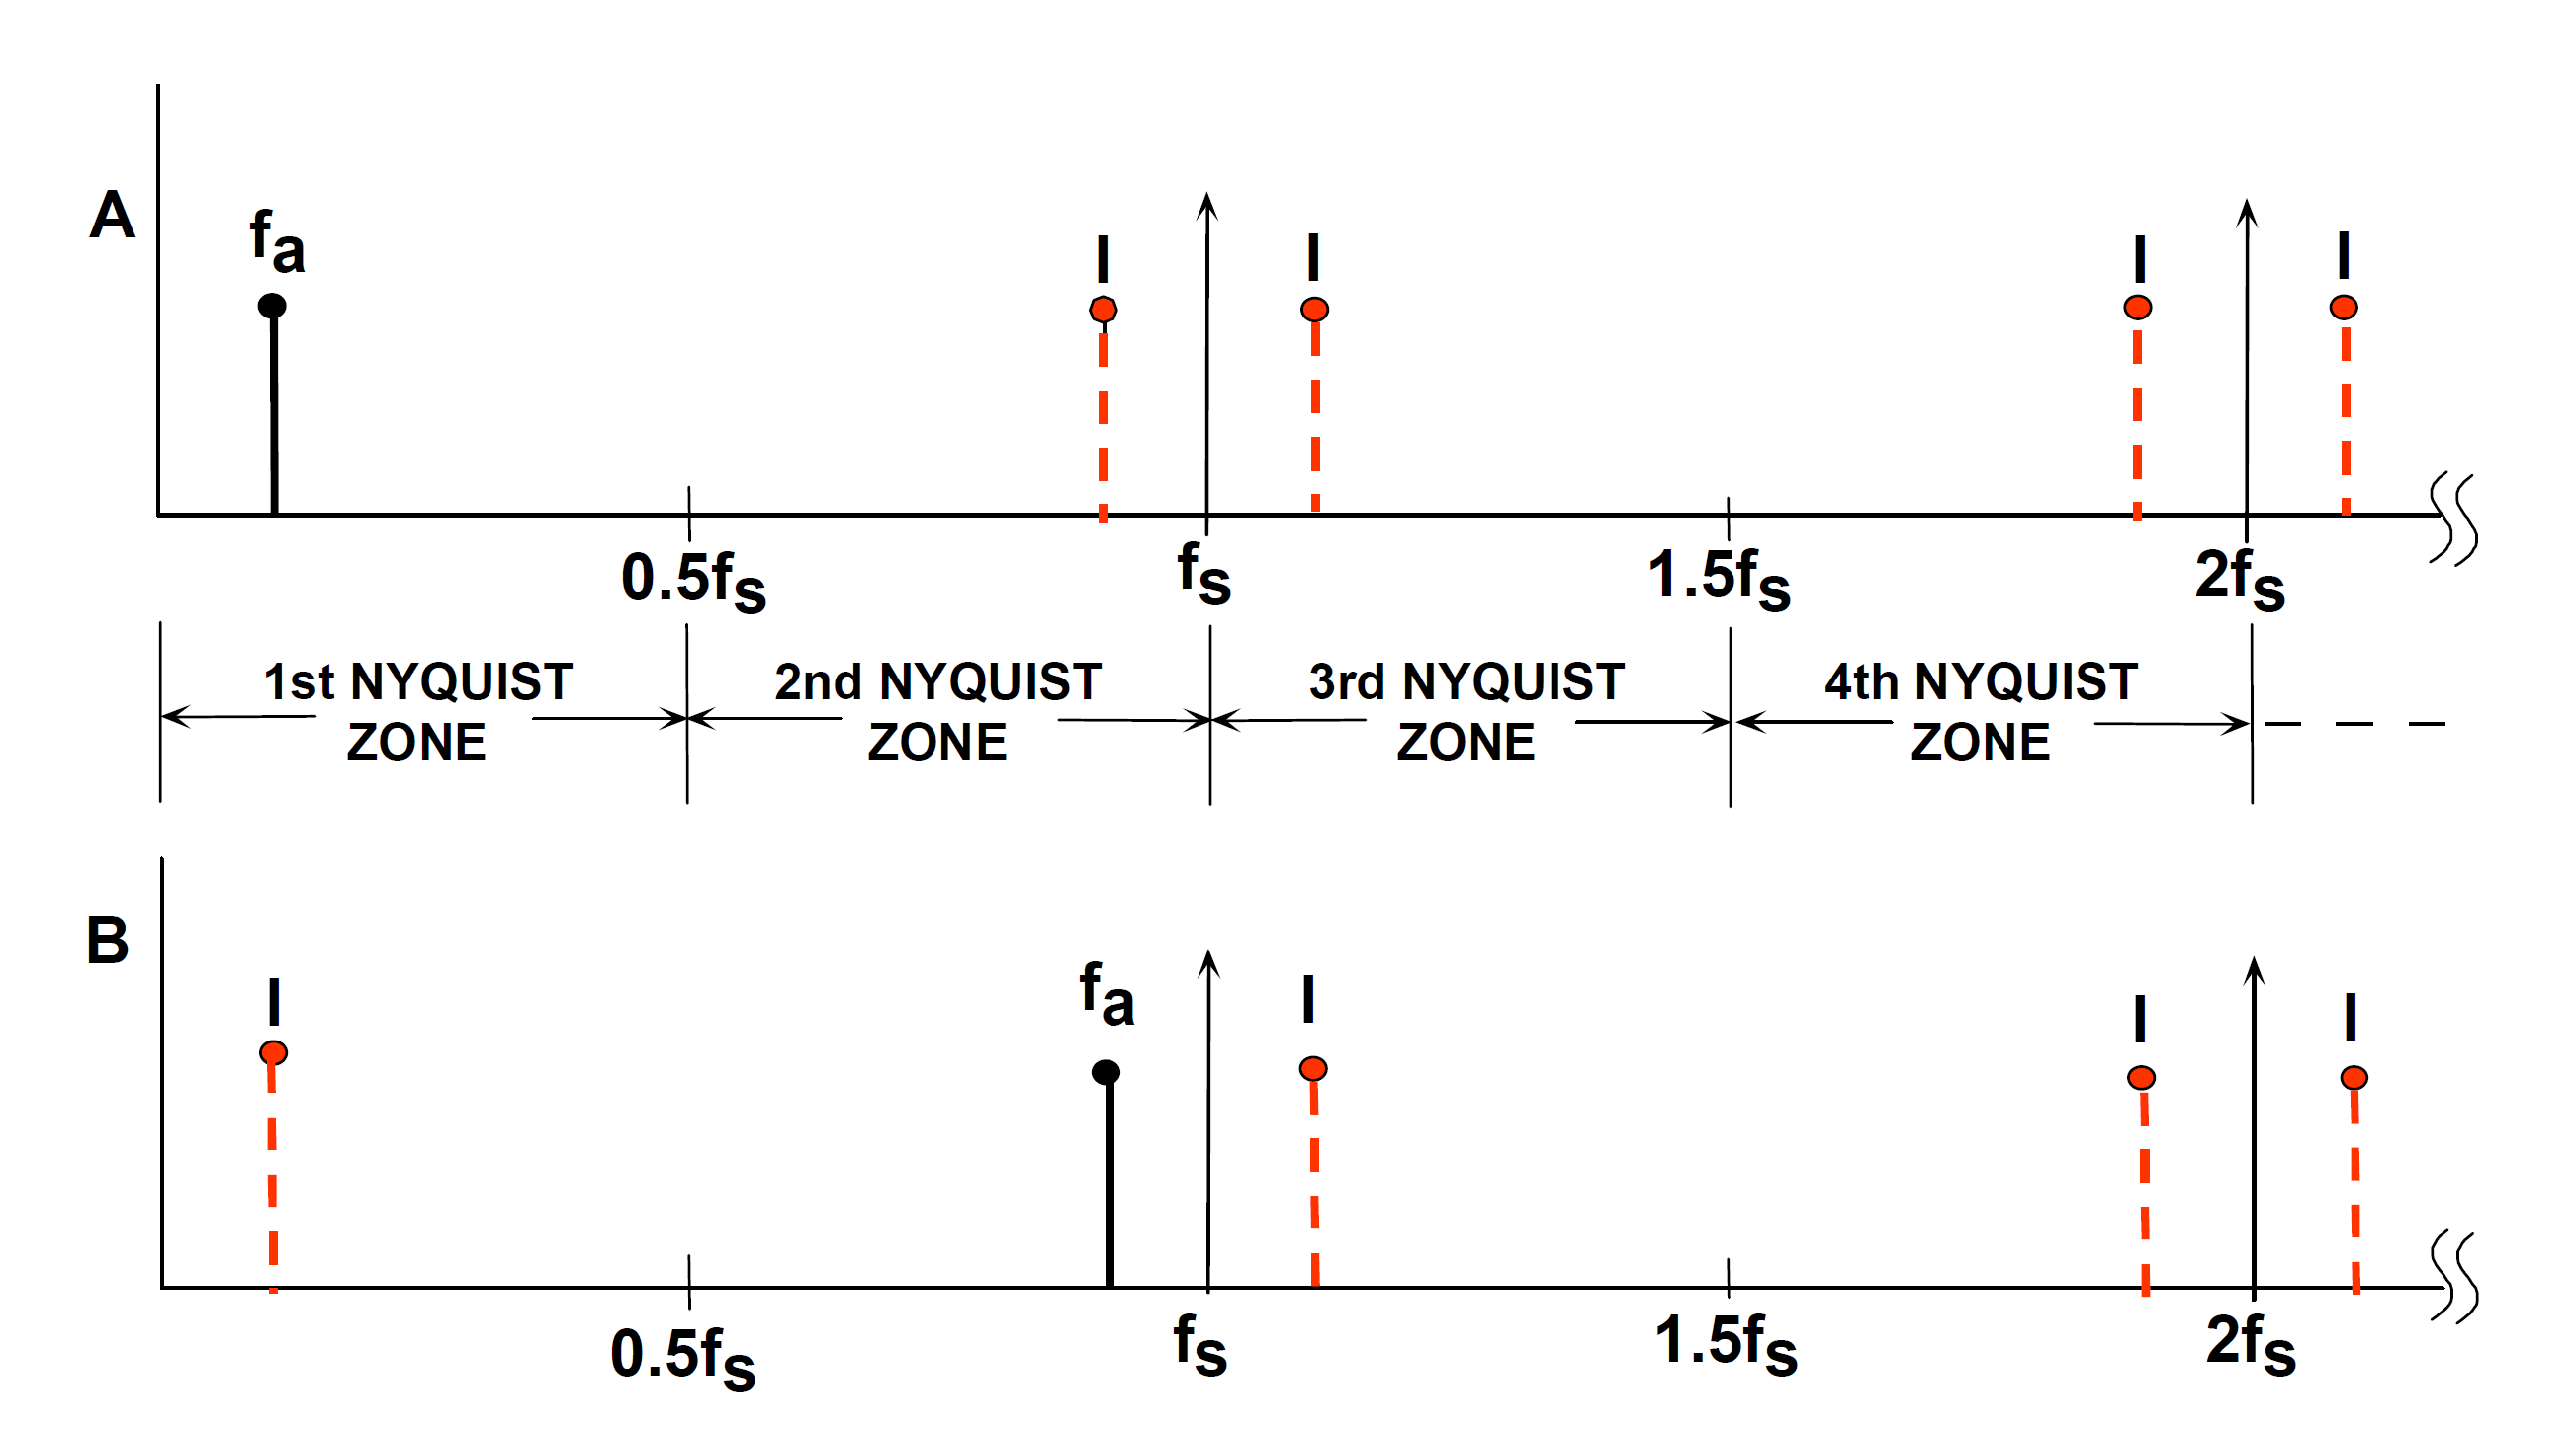
\includegraphics[width=\linewidth]{chap/02-theory/img/alias_f}  
		\caption{Sampling in frequency domain}
		\label{fig:alias_f}
	\end{subfigure}
	\begin{subfigure}{\textwidth}
		\centering
		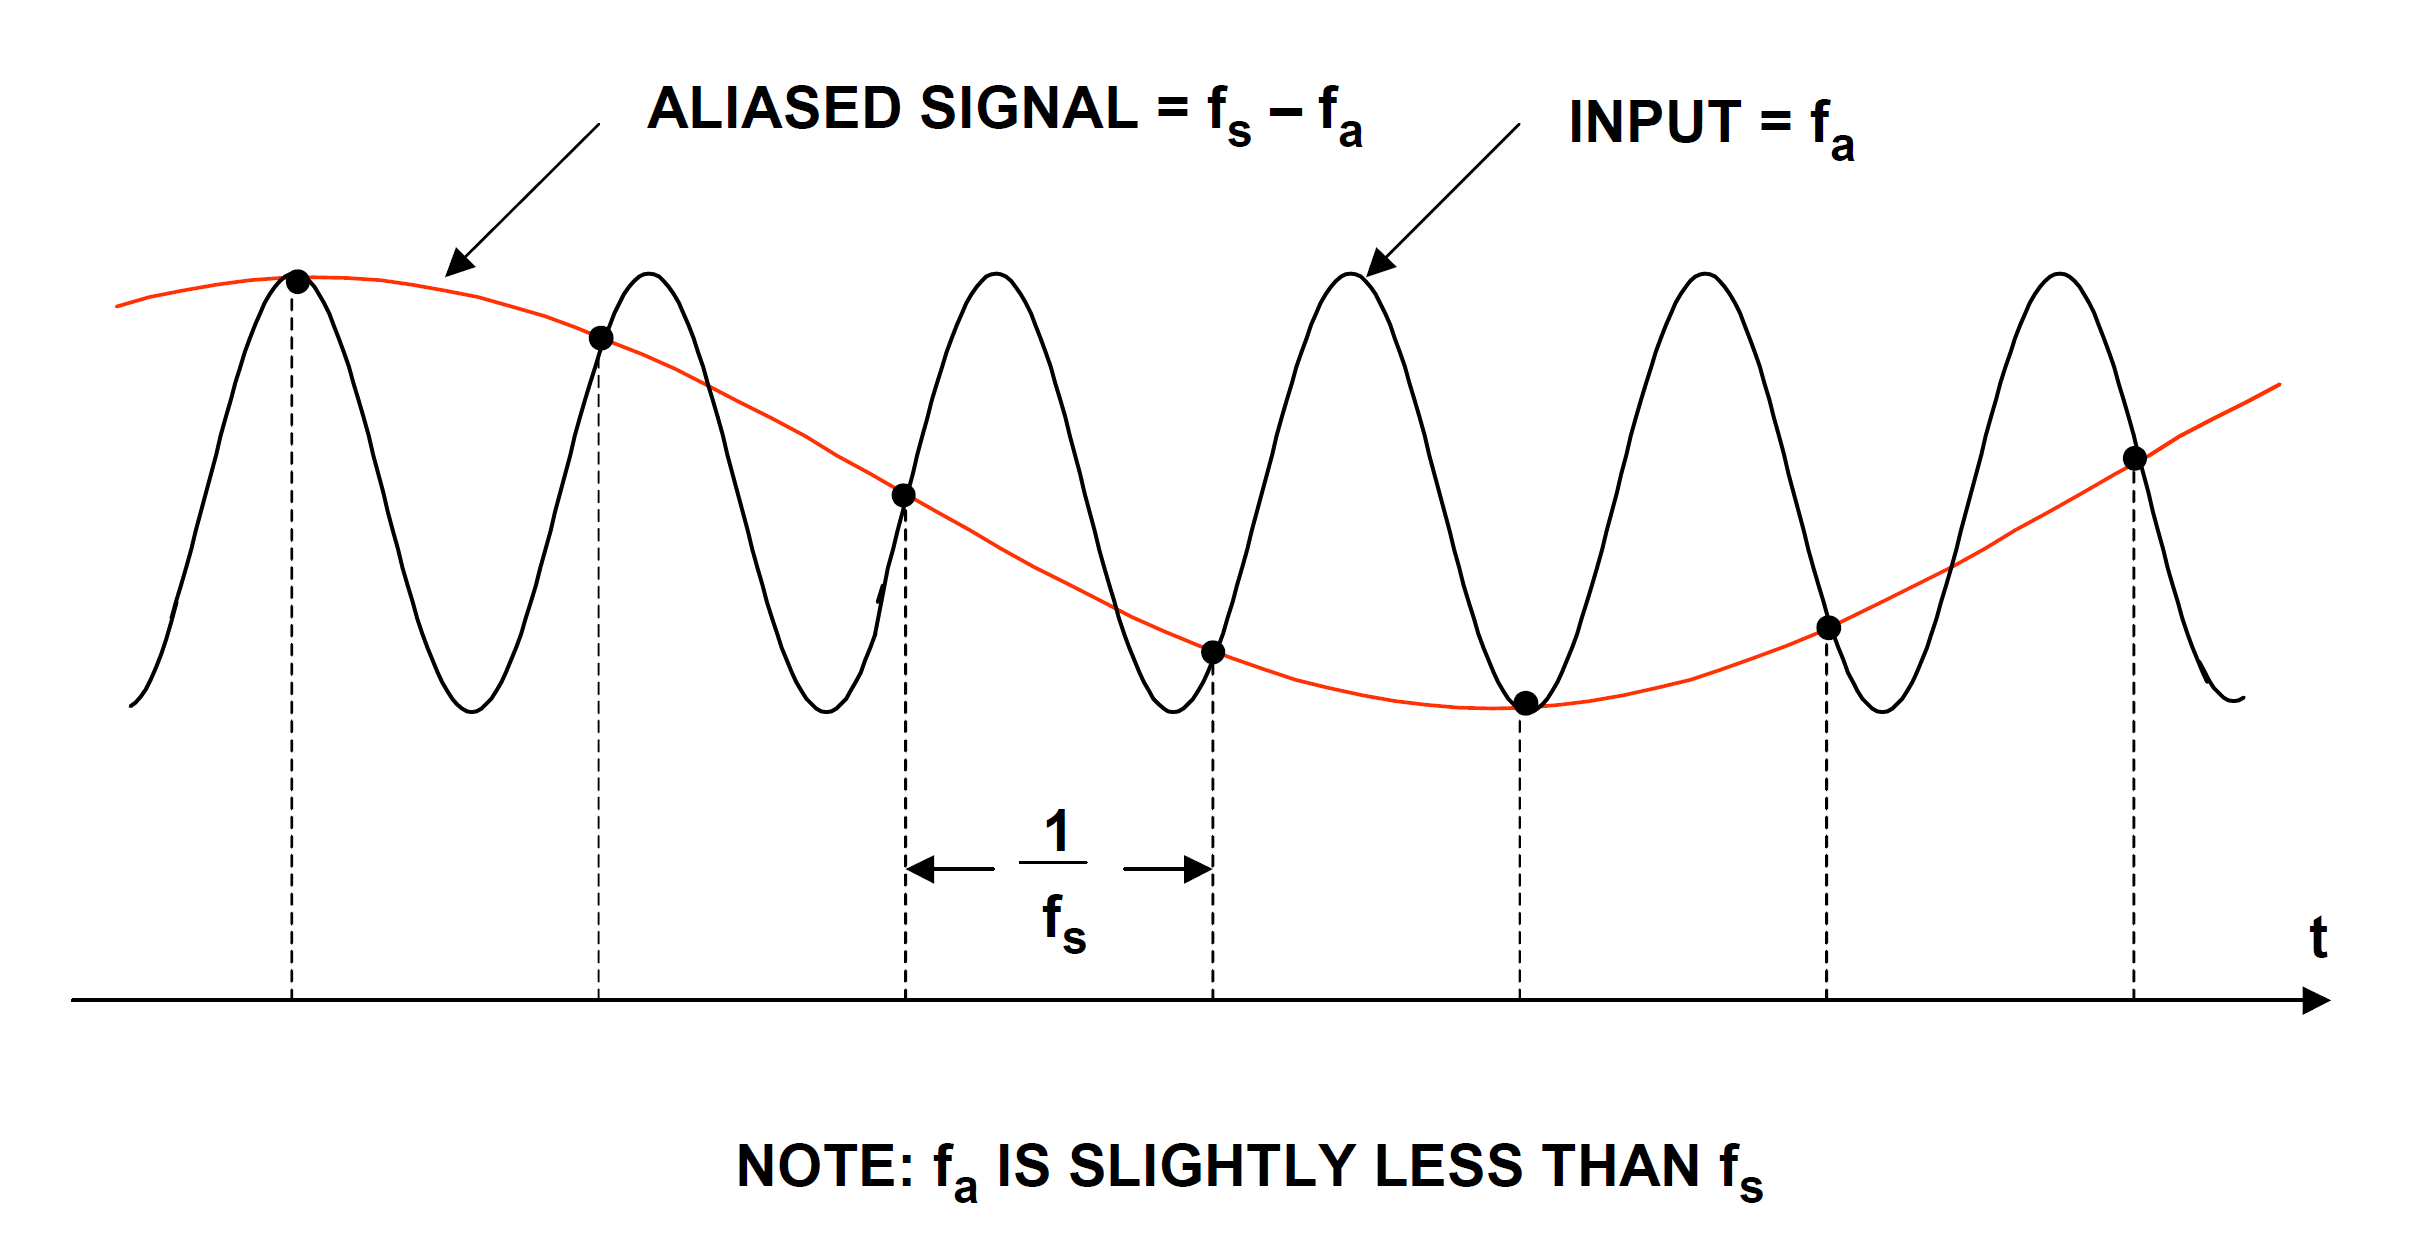
\includegraphics[width=\linewidth]{chap/02-theory/img/alias_t}  
		\caption{Aliasing in time domain}
		\label{fig:alias_t}
	\end{subfigure}
	\caption[Aliasing]{Analog signal with frequency $f_a$ sampled at $f_s$ respecting (A) and not respecting (B) the Nyquist criteria. \autoref{fig:alias_t} shows the effect of case B in time domain. \cite{walt}}
\end{figure}
%todo to tikz
%todo explain nyquist-bandwidth
%todo low-pass filter to get B/2<f_s? maybe


\paragraph{Sample-And-Hold-Amplifier}
\Glspl{adc} need a certain amount of time to sample the input signal.
If the level of the analog signal changes by more than one \gls{lsb} during this period, this can result in large errors in the output signal.
Therefore, so called \gls{sha} are used in front of the \gls{adc} to hold the input level constant for the needed amount of time.
The \gls{adc} sampling time needs to be timed in such way, that the analog-to-digital conversion falls into the hold period of the \gls{sha} and does not exceed into the sample period, for example like shown in \autoref{fig:sha_sampling}. Thus, the upper frequency limitation is not determined by the \gls{adc} itself, but rather by the aperture jitter, bandwidth, distortion, etc. of the \gls{sha}. \cite{walt}

\begin{figure} [H]
	\centering
	\tikzexternaldisable
	\includegraphics[width=\linewidth]{chap/02-theory/img/sha_timing}  
	\caption{Example for appropriate sampling timing when using Sample-And-Hold-Amplifier}
	\label{fig:sha_timing}
	\tikzexternalenable
\end{figure}
%todo why not save this as .tikz file and include it as a normal figure with caption?

In addition to the \gls{sha}, there is also the \gls{tha}.
Instead of a sample period, the \gls{tha} has a track period, where the output of the amplifier tracks the input signal (see also \autoref{fig:tha}).
When switching to hold mode, the signal at this instant is held. This is opposed to the \gls{sha}, where the output during sample mode is actually not defined and is set to the value of the input signal, only when switching into hold mode. In the track mode interval of the output waveform (positive differential clock voltage), the device behaves as a unity-gain amplifier that replicates the input signal at the output stage, subject to the input bandwidth and the output amplifier bandwidth limitations. At the positive to negative clock transition of the device, it samples the input signal with a very narrow sampling time aperture and holds the output relatively constant during the negative clock interval at a value that is representative of the signal at the instant of sampling. \cite{Reeder2019}
%todo explanation a bit confusing. use another timing diagram?

\begin{figure}[tbh]
	\centering
	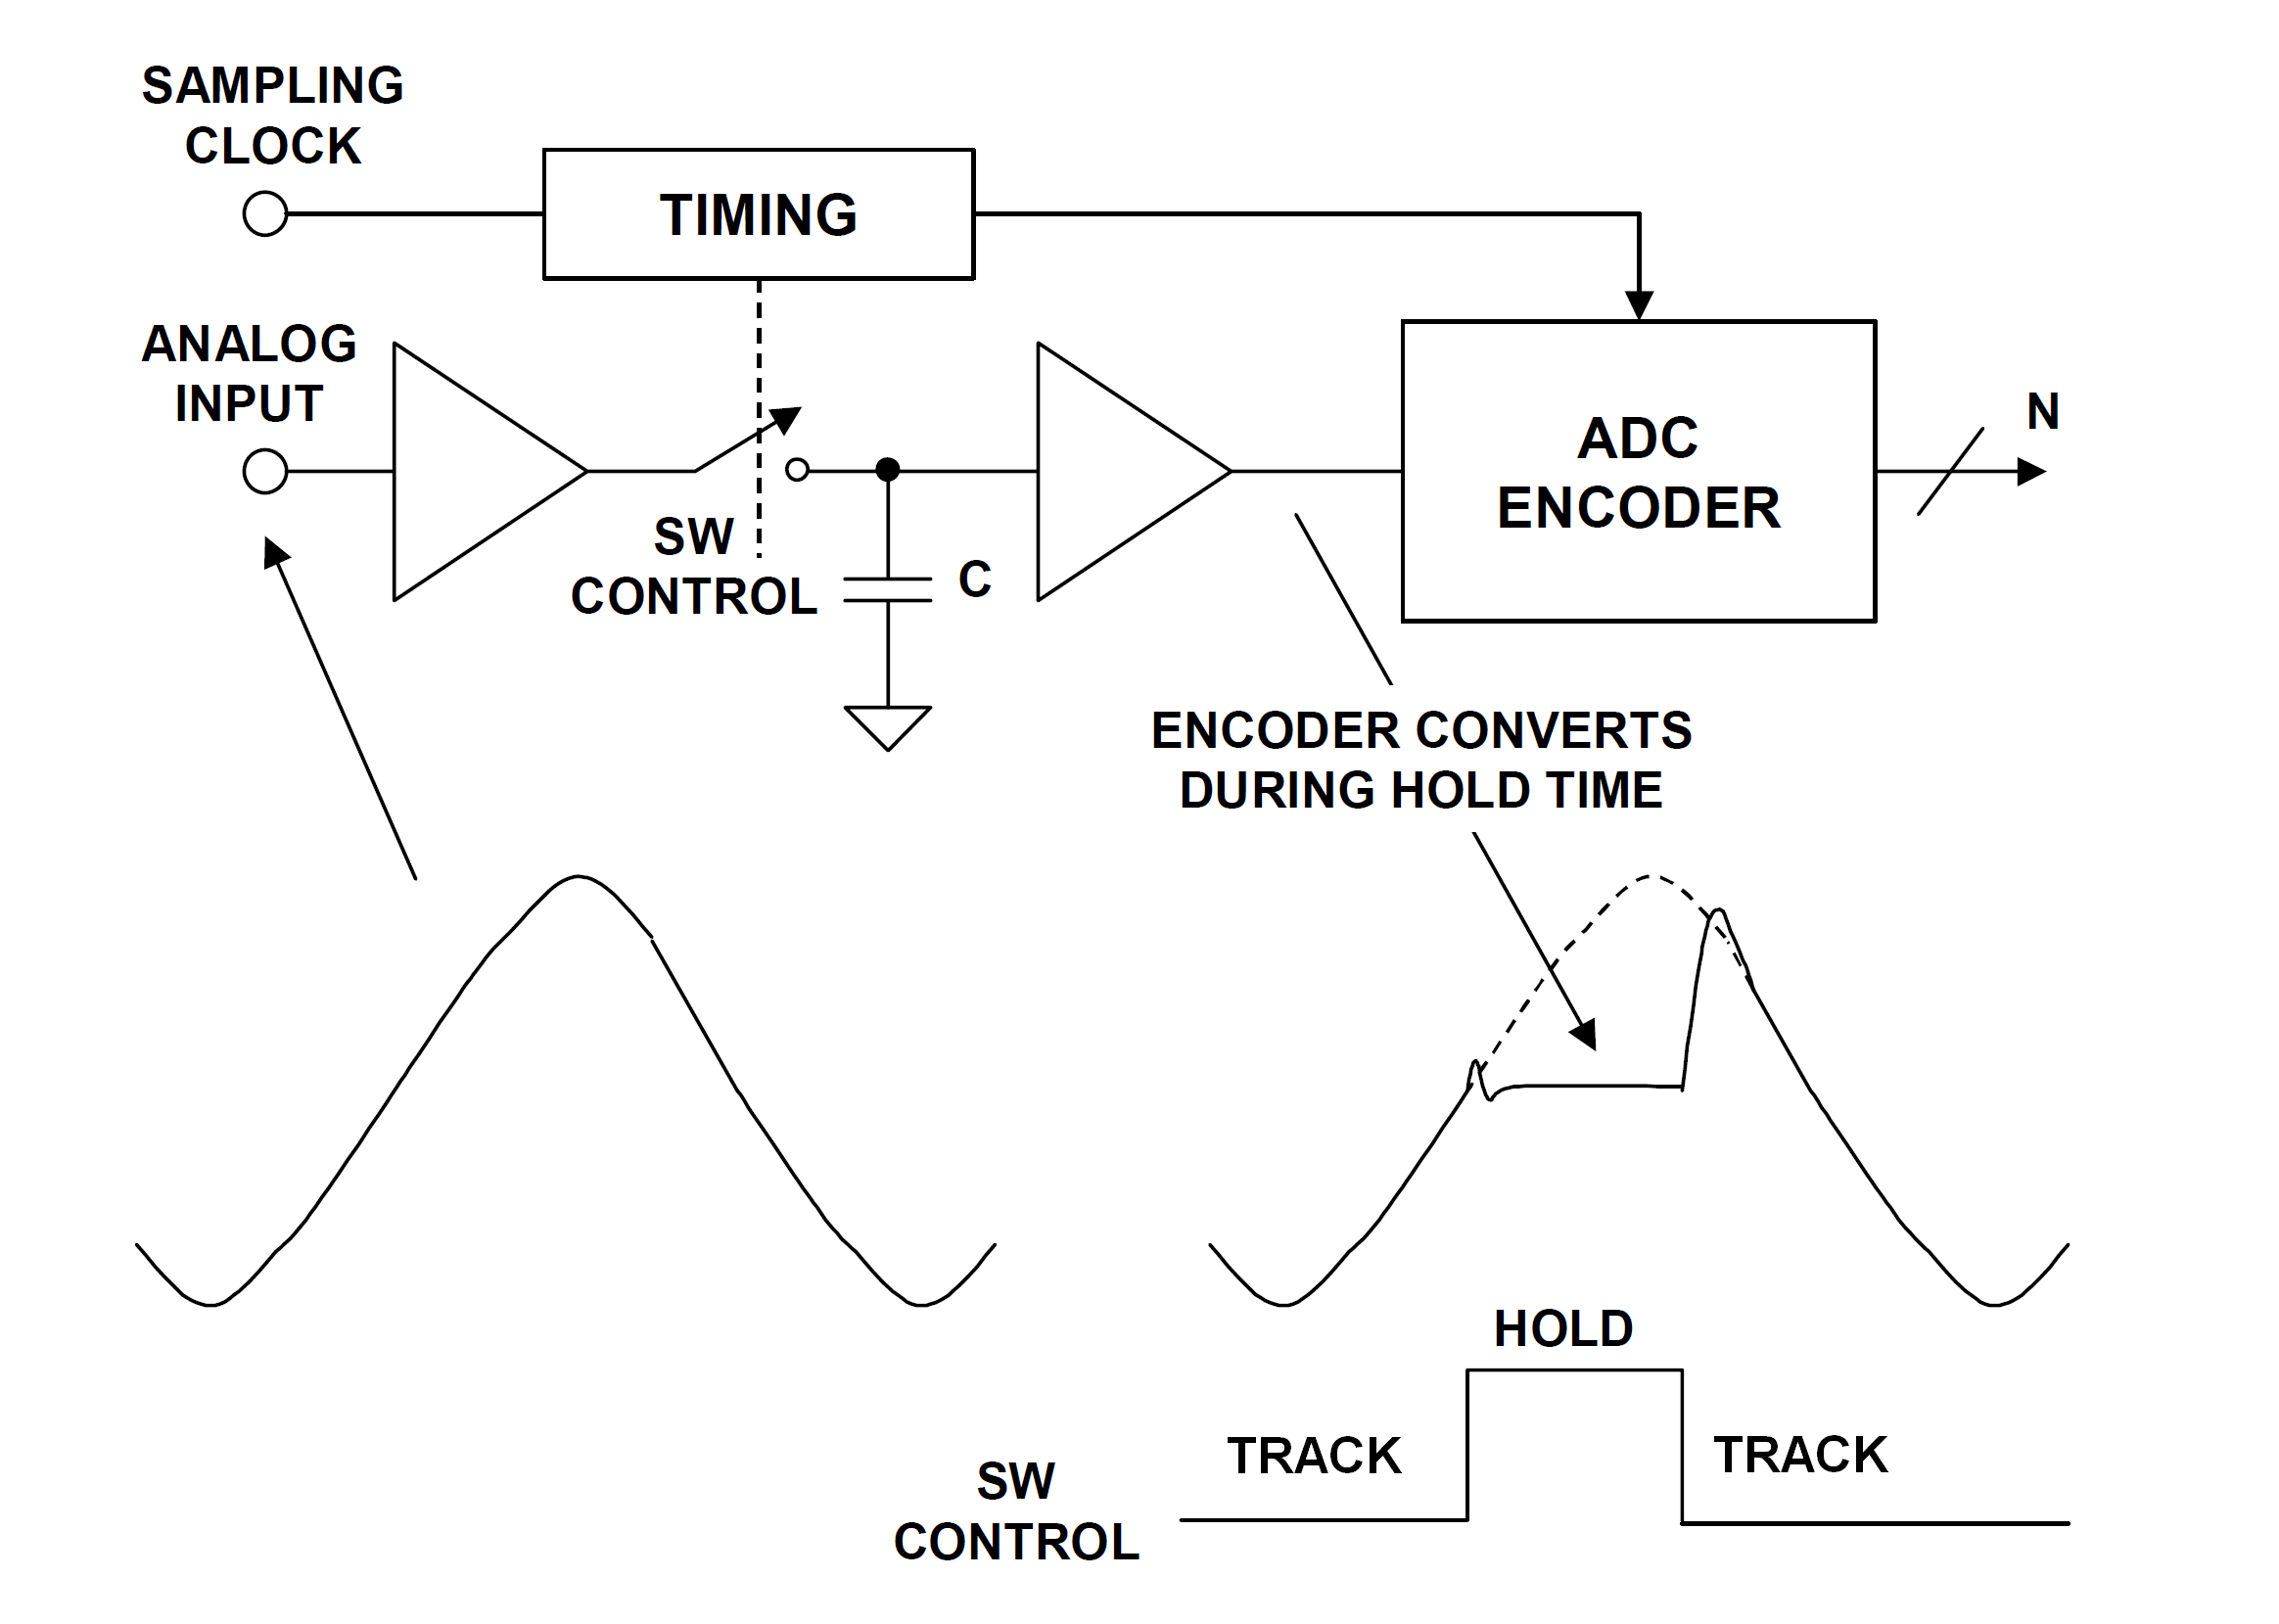
\includegraphics[width = \textwidth]{chap/02-theory/img/tha}
	\caption{Track-And-Hold-Amplifier schematic and principle \cite{walt}}
	\label{fig:tha}
\end{figure}

\subsubsection*{Characteristics of Analog-To-Digital-Converters} 
For an ideal converter, the number of bits would be sufficient to fully characterize it.
Real \glspl{adc} however differ from the ideal behavior by introducing static and dynamic imperfections.
Different applications have different requirements, which leads to a number of specifications.
These can be divided into the following categories \cite{Lundberg}:
\begin{itemize}[noitemsep]
	\item Quantization Noise
	\item Static parameters
	\item Frequency-domain dynamic parameters
	\item Time-domain dynamic parameters
\end{itemize}
This section provides an overview of these figures of merit.
Which of these are needed to specify the necessary performance of the \gls{adc} has to be chosen for each application accordingly.

\paragraph{Quantization Noise}\label{par:quant_noise}
Even in an ideal $N$-bit converter there will be errors during the quantization, which behave like noise.
The reason is that each $N$-bit word represents a certain range of analog input values, which is 1 \gls{lsb} wide and centered around a code center (see \autoref{fig:idealADC}) \cite{Lundberg}.
The input voltage is assigned to the word of the nearest code center.
This means that there will always be a difference between the corresponding voltage of the respective digital code $x_q(t)$ and the actual analog input voltage  $x(t)$.
This difference is called the \textit{quantization error}. For an equidistant quantization, the quantization error for a code width $q$ is (see \cite{puente2015})
\begin{equation}
\left| e_q(t) \right| = \left| x(t) - x_q(t) \right| \leq \frac{q}{2}.
\end{equation}

Assuming the error voltage uncorrelated and uniformly distributed, the theoretical (maximum) \gls{snr} of this \textit{quantization noise} can be calculated. In the time domain, the quantization error $e(t)$ can be approximated with a sawtooth signal: %todo uncorrelated to what other signal?
\begin{equation}
e(t) = st, \quad -\frac{q}{2s} < t < \frac{q}{2s} 
\end{equation}
\begin{figure}[tbh]
	\centering
	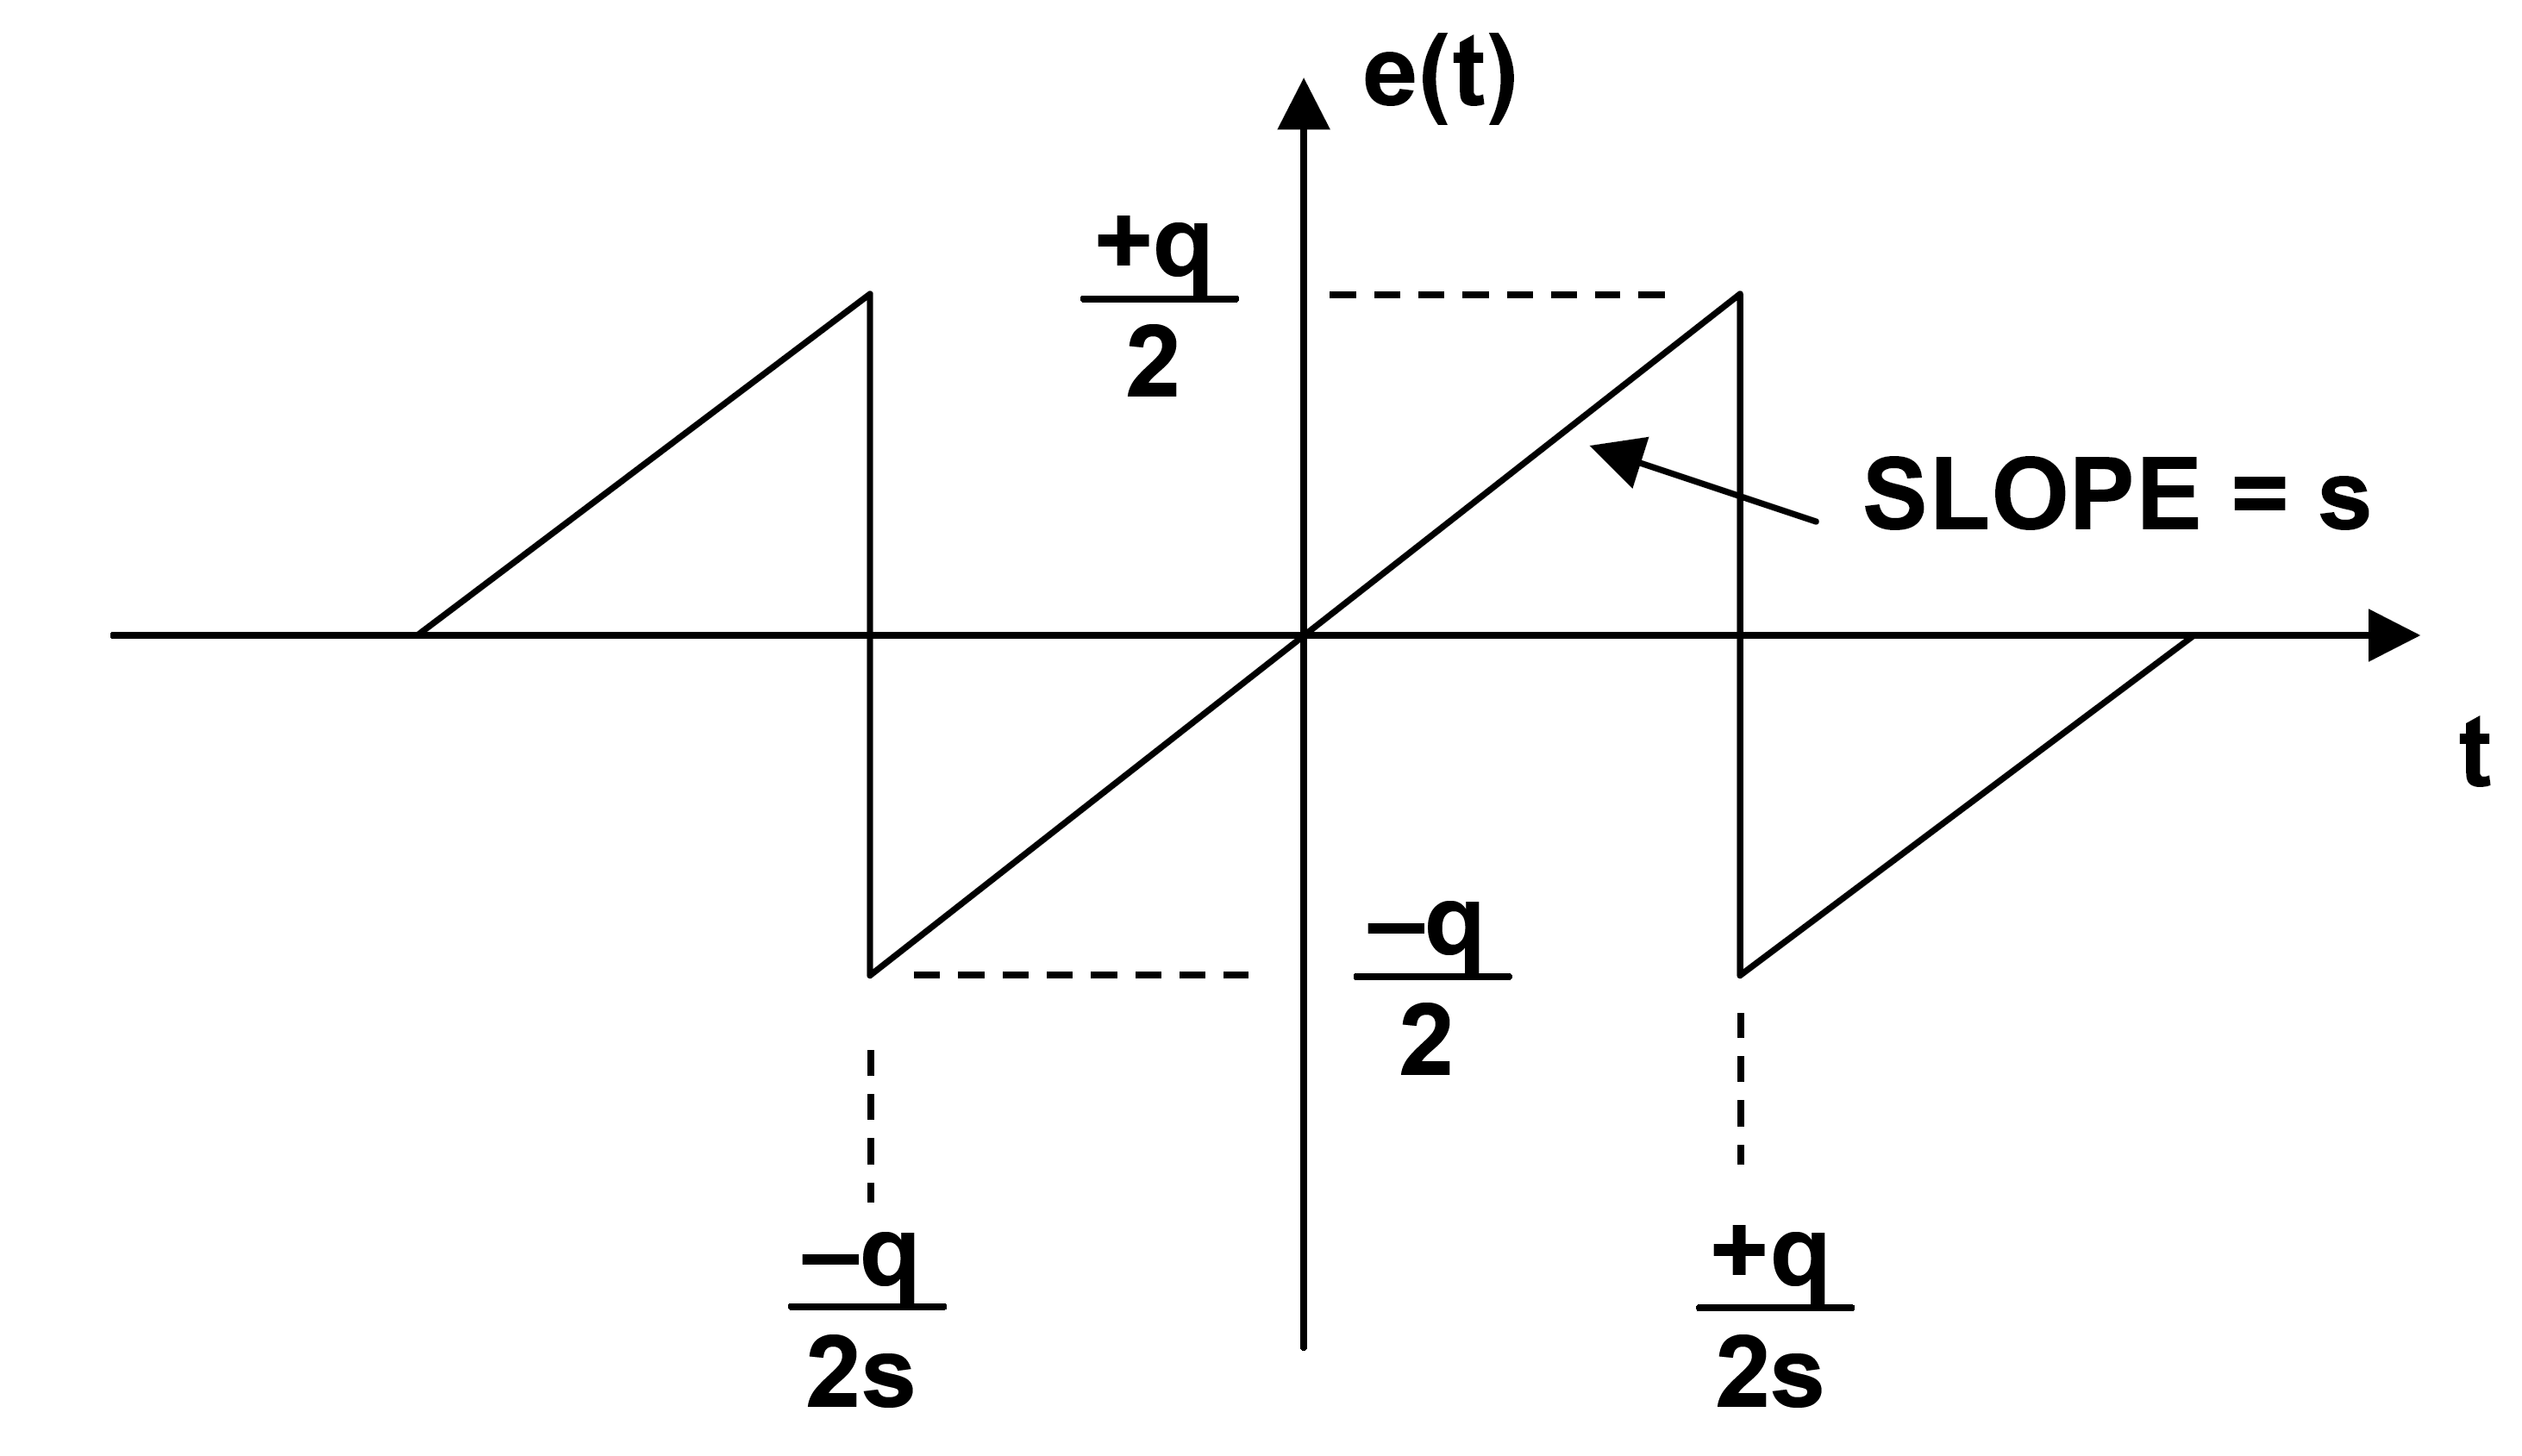
\includegraphics[width = 0.7\textwidth]{chap/02-theory/img/quantization_error.tikz}
	\caption{Quantization noise as function of time (redrawn from \cite{walt})}
	\label{fig:eq}
\end{figure}

The power of the quantization noise, which is assumed to be uncorrelated and broadband, can be calculated as the mean-square $e_{\text{rms}}^2$of $e(t)$ \cite{walt}:
\begin{equation}
P_{QN} = e_{\text{rms}}^{2} = \overline{e^{2}(t)} = \frac{s}{q}\int_{-q/2s}^{+q/2s} (st)^{2} dt = \frac{s^3}{q} \left[ \frac{t^3}{3}\right]_{-\frac{q}{2s}}^{+\frac{q}{2s}} = \frac{q^2}{12}
\end{equation}
%todo again uncorrelated to what. and it sounds like the power has correlation

To calculate the maximal \gls{snr} of an ideal converter, a full-scale input sine wave is assumed:
\begin{equation}
u(t) = u_s \sin(2\pi f t) = \frac{2^{N}q}{2}\sin(2\pi f t)  = 2^{N-1}q \sin(2\pi f t)
\end{equation}
With the effective value of the signal amplitude
\begin{equation}
u_{\text{eff}} = \frac{u_s}{\sqrt{2}} = \frac{2^{N-1}q}{\sqrt{2}}
\end{equation}
\gls{snr}
\begin{equation}
\text{SNR} = \frac{P_{\text{signal}}}{P_{\text{noise}}} = \frac{u_{\text{eff}}^{2}}{e_{\text{rms}}^{2}} = \frac{2^{2N-2}q^2/2}{q^2/12} = 2^{2N} \cdot 1.5.
\end{equation}
In decibel:
\begin{equation}\label{eq:idealSNR}
\text{SNR}|_{\text{dB}} = 10\log\left(2^{2N}\cdot 1.5\right) = 6.02 N + 1.76
\end{equation}
\cite{puente2015} \cite{walt}



\paragraph{Static parameters}
\textit{Static parameters} are specifications, which can be measured at low speed/DC. 
\paragraph{Accuracy}
\textit{Accuracy} is the total error with which an \gls{adc} can convert a known voltage, which includes the effects of:
\begin{itemize}[noitemsep]
	\item Quantization error
	\item Gain error
	\item Offset error
	\item Nonlinearities
\end{itemize}
\cite{Lundberg}
\paragraph{Resolution}
\textit{Resolution} is the number of bits $N$ of the \gls{adc}.
Depending from the resolution are the size of the \gls{lsb}, which in its turn determines the dynamic range, code widths and quantization error.
\paragraph{Dynamic Range}
The \textit{dynamic range} represents the ratio between smallest possible output (\gls{lsb} voltage) and the largest possible output (full-scale voltage).
It can be calculated as
\begin{equation}
	20 \log 2^{N} \approx 6N.
\end{equation}

\paragraph{Offset and Gain Error}
The \textit{offset error} is the deviation of the first transition voltage from the ideal $1/2$ \gls{lsb}.
%todo 'first'?

\textit{Gain Error} defines the deviation of the slope of the line going through the zero and full-scale point of the transfer function. %todo state eq for 'transfer function' otherwise 'line', 'zero' and 'full-scale point' undefined here

These errors can easily be corrected by calibration.
\autoref{fig:offsetErr} visualizes the effects of both offset and gain error. 
\begin{figure}[tbh]
	\centering
	\includegraphics[width = 0.7\textwidth]{chap/02-theory/img/offset_err.tikz}
	\caption[Effects of Offset and Fain error in ADC]{Offset and Gain Error in the \gls{adc} characteristic transfer function. Notice the difference between the line going through the code centers (dashed) and the line of an ideal \gls{adc} (dotted)}
	\label{fig:offsetErr}
\end{figure}
%todo where is this full-scale point here in the fig?

\paragraph{Integral and Differential Non-linearity Distortion} 
\textit{\gls{inl}} in the transfer function is the distance of the code centers from the ideal line. %todo which transfer function?
It results from the integral non-linearities of the front-end, \gls{sha} and also the \gls{adc} itself. \cite{walt} These nonlinearities depend on the input signal amplitude. \cite{Lundberg}
%todo not sure about the \textit + \gls

\textit{\gls{dnl}} is the deviation in code width from the ideal width of 1 \gls{lsb}. This nonlinearity stems exclusively from the encoding process in the \gls{adc}. \cite{walt}
It not only depends on the input signal amplitude, but also on the positioning along the transfer function. \cite{Lundberg} %todo what do you mean by position?

\begin{figure}[tbh]
	\centering
	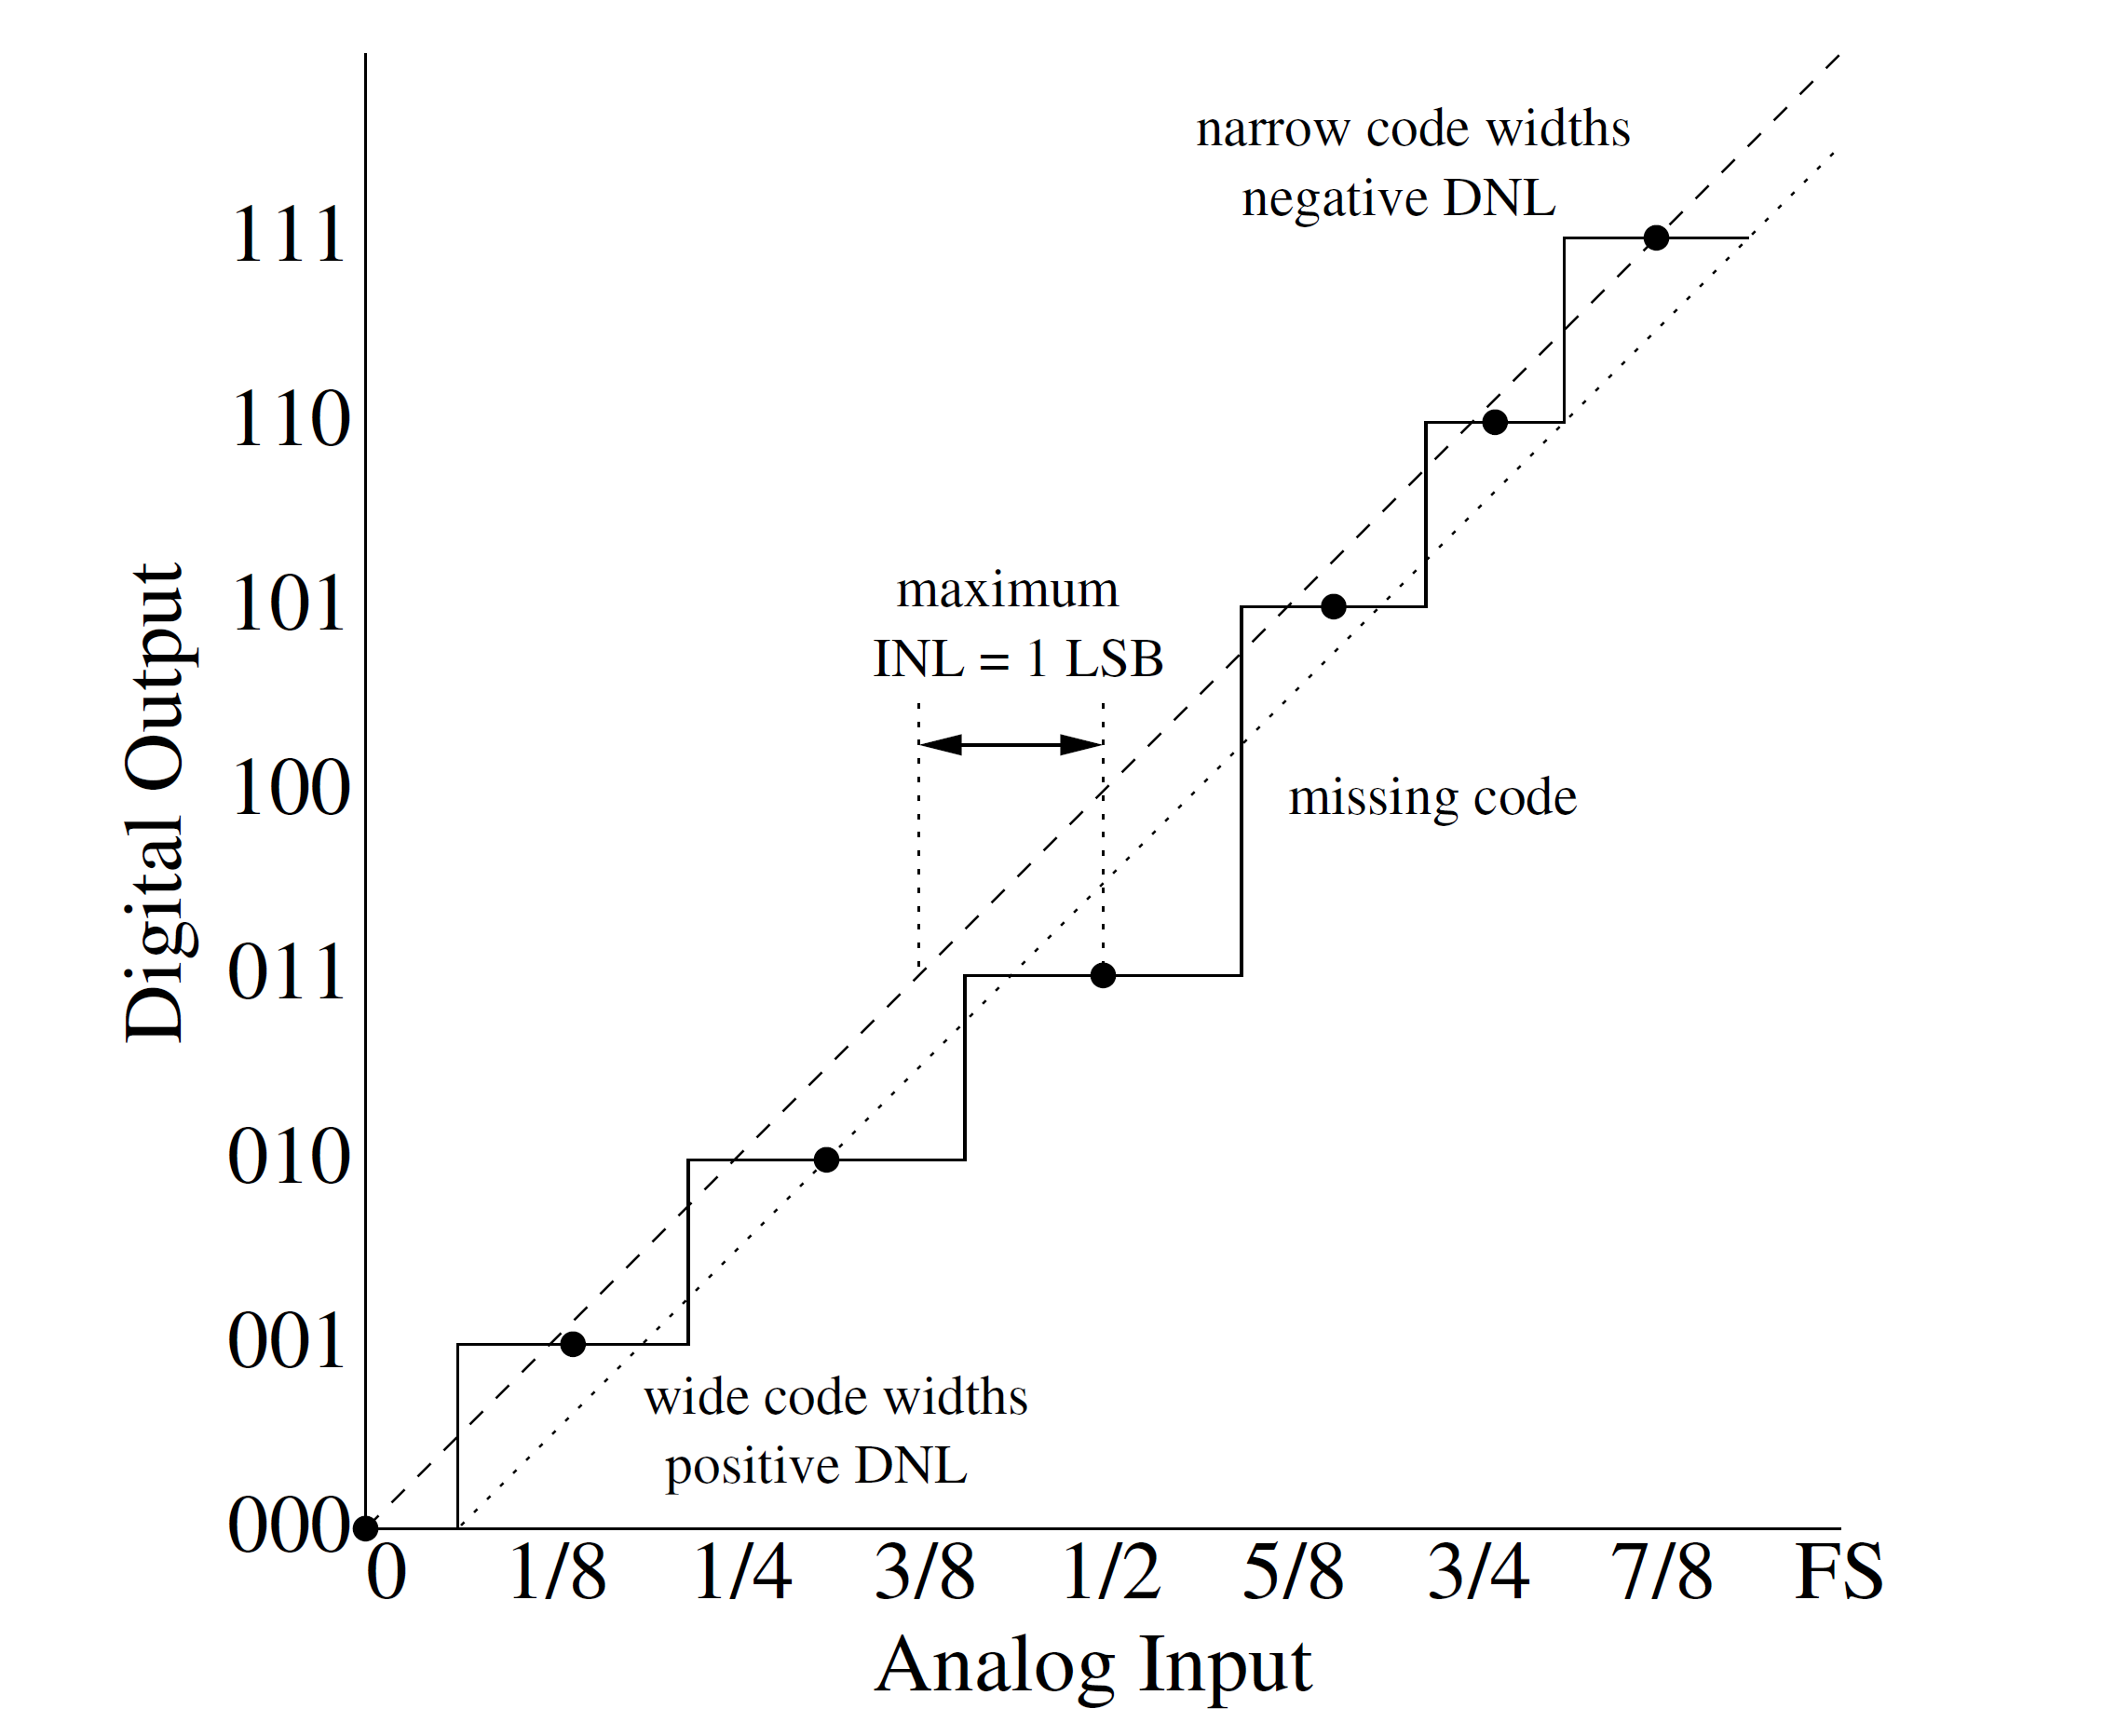
\includegraphics[width = 0.7\textwidth]{chap/02-theory/img/dnld}
	\caption{Placeholder: Integral and Differential Nonlinearity Distortion \cite{Lundberg}}
	\label{fig:nld}
\end{figure}
%todo to tikz

\paragraph{Frequency-Domain Dynamic Parameters}
Any real \gls{adc} is subject to noise distortion.
\textit{Noise} includes any unwanted (random or deterministic) signal components, which interfere with the measuring of the desired signal. Examples are quantization noise or random fluctuations due to thermal noise.

\textit{Distortion} is the term for the change of the original signal. %todo not sure if that's the correct definition. definetely cite so here.

In an \gls{adc} (with built-in \gls{sha}) there are a couple of sources, which introduce noise and distortion:
\begin{itemize}
	\item \textbf{Input Stage:} Wideband noise, non-linearity and bandwidth limitation
	\item \textbf{\gls{sha}:} Non-linearity, aperture jitter(see paragraph about Time-Domain Dynamic Performances)  and bandwidth limitation
	\item \textbf{\gls{adc}:} Quantization noise, non-linearity
\end{itemize}

In the following, an overview of the metrics for quantification of these imperfections is given. 
%todo are those sub-paragraphs? (maybe promote \paragraph{Frequency-Domain Dynamic Parameters})
%todo orrrr just make a big itemmize with all the following very short paragraphs

\paragraph{Signal-to-Noise-and-Distortion Ratio}
\textit{\gls{sinad}} (also called SNDR or S/N+D) denotes the ratio between the \gls{rms} of the signal amplitude to the mean value of the Root-Sum-Square (RSS) of all other spectral components, including harmonics, but excluding  DC (\SI{0}{\hertz}). \gls{sinad} is a good indication over the general dynamic performance of the \gls{adc}, as it includes all contributions from noise and distortion.

\paragraph{Effective-Number-Of-Bits}
The \textit{\gls{enob}} expresses the \gls{sinad} in terms of bits. It can be calculated as
\begin{equation}
	\text{ENOB} = \frac{\text{SINAD}-\SI{1.76}{\decibel}}{\SI{6.02}{\decibel}/\text{bit}}. \quad \cite{walt2009}
\end{equation}
This is derived from solving the equation of the "ideal \gls{snr}" \autoref{eq:idealSNR} for the number of bits $N$ and substituting \gls{snr} with \gls{sinad}. This however means, that this parameter assumes a full-scale input signal. Expressing the \gls{enob} for a smaller signal amplitude requires measuring the \gls{sinad} at this level and a correction factor. \cite{walt}

\paragraph{Spurious-Free Dynamic Range}
\textit{\gls{sfdr}} indicates the dynamic range of the converter, which can be used, before there is interference or distortion from spurious components with the fundamental signal. \cite{Lundberg} The \gls{sfdr} is calculated as the \gls{rms} value of the fundamental signal to the \gls{rms} value of the worst spurious signal, i.e. the highest spur in the spectrum. It is measured over the whole Nyquist-Bandwidth (DC (\SI{0}{\hertz}) to $f_s/2$, $f_s$ being the \gls{adc} sampling rate). The spur may or may not be a harmonic of the fundamental signal. \cite{walt2009} \cite{Lundberg}

The \gls{sfdr} is an important characteristic in the sense, that it indicates the smallest signal which can still be distinguished from a strong interfering signal. \cite{walt2009} 

\autoref{fig:sfdr} illustrates the \gls{sfdr} in terms of \gls{dbfs} and \gls{dbc}.

\begin{figure}[tbh]
	\centering
	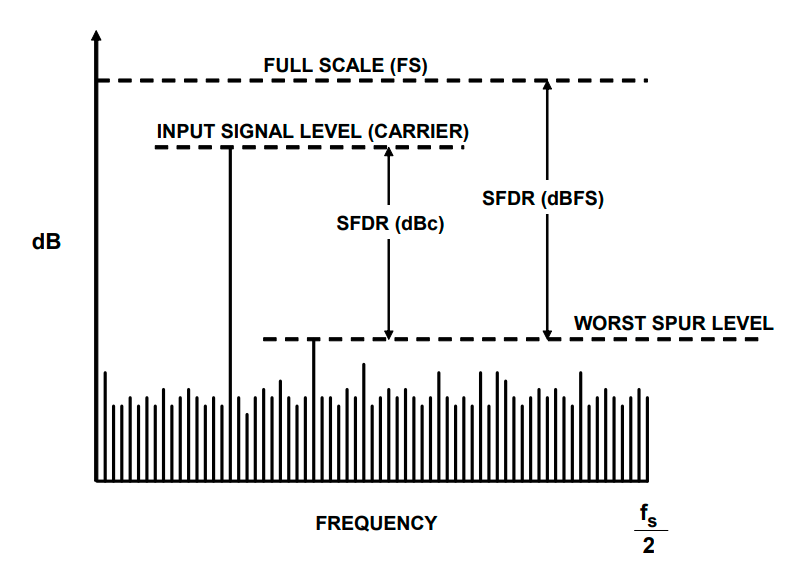
\includegraphics[width = \textwidth]{chap/02-theory/img/sfdr}
	\caption{Placeholder: SFDR \cite{walt2009}}
	\label{fig:sfdr}
\end{figure}
%todo to tikz
\paragraph{Total Harmonic Distortion}
The \textit{Total Harmonic Distortion} describes the ratio of the \gls{rms} sum of the first five harmonic components (or aliased versions of them) to the \gls{rms} of the considered fundamental signal. \cite{Lundberg}

\paragraph{Effective Resolution Bandwidth}
\textit{Effective Resolution Bandwidth} denotes the frequency of the input signal, at which the \gls{sinad} has fallen by \SI{3}{\decibel} ($\eqdev$ 0.5 bit in terms of \gls{enob}) compared to the \gls{sinad} at lower frequency range. \cite{Lundberg}

\paragraph{Analog Input Bandwidth}
\textit{Analog Input Bandwidth} is the analog input frequency at which the power of the fundamental is reduced by 3dB with respect to the low-frequency value.

\paragraph{Full-Linear Bandwidth}
The \textit{Full-Linear Bandwidth} is defined as the frequency at which the slew-rate (SR) of the \gls{sha} starts to distort the input signal by a specified value. \cite{Lundberg} The slew-rate is defined as the rate of how much the voltage $v$ changes against time $t$:
\begin{equation}
	\text{SR} = \frac{dv}{dt}
\end{equation}
A SR of \SI{1}{\volt \per \micro \second} for example means, that the output of the amplifier can not change more than \SI{1}{\volt} over the course of \SI{1}{\micro \second}.\cite{2021Slew} 

\paragraph{Time-Domain Dynamic Parameters}
Time-Domain Dynamic parameters describe the deviation of the converter's behavior from the ideal one in time domain. 

\paragraph{Aperture Delay}
\textit{Aperture Delay} (or \textit{aperture time}) is defined as delay between the triggering of the converter (e.g. rising edge of the sampling clock) and the actual conversion of the input voltage into the digitized value. \cite{Lundberg}

\paragraph{Aperture Jitter}
\textit{Aperture jitter} describes the sample-to-sample variation in aperture delay. Jitter can cause significant error in the voltage and decreases the overall \gls{snr} of a converter. Especially for high-speed \glspl{adc} jitter poses a limit in performance.

Assuming a full-scale sinus-wave $V_{\text{in}}$ as input signal with 
\begin{equation}
	V_{\text{in}} = V_{\text{FS}} \sin (\omega t)
\end{equation}
the maximal slope of this signal is then
\begin{equation}
	\frac{dV_{\text{in}}}{dt}\Bigr|_{\text{max}} = \omega V_{\text{FS}}
\end{equation}
Aperture jitter $\Delta t_{\text{rms}}$ occuring during the sampling of this maximal slope produces the \gls{rms} voltage error 
\begin{equation}
	\Delta V_{\text{rms}} = \omega  V_{\text{FS}} \Delta t_{\text{rms}} = 2 \pi f  V_{\text{FS}} \Delta t_{\text{rms}}.
\end{equation}
As variations in aperture time occur randomly, these errors behave like a random noise source. This way, a \gls{sjnr} can be defined as
\begin{equation}
	\text{SJNR} = 20 \log \left( \frac{V_{\text{FS}}}{\Delta V_{\text{rms}}} \right) = 20 \log \left( \frac{1}{2 \pi f  V_{\text{FS}}} \right)
\end{equation}

The voltage error due to jitter and the \gls{sjnr} for different aperture jitter values are shown in \autoref{fig:ap_jit}.

\begin{figure}[tbh]
	\centering
	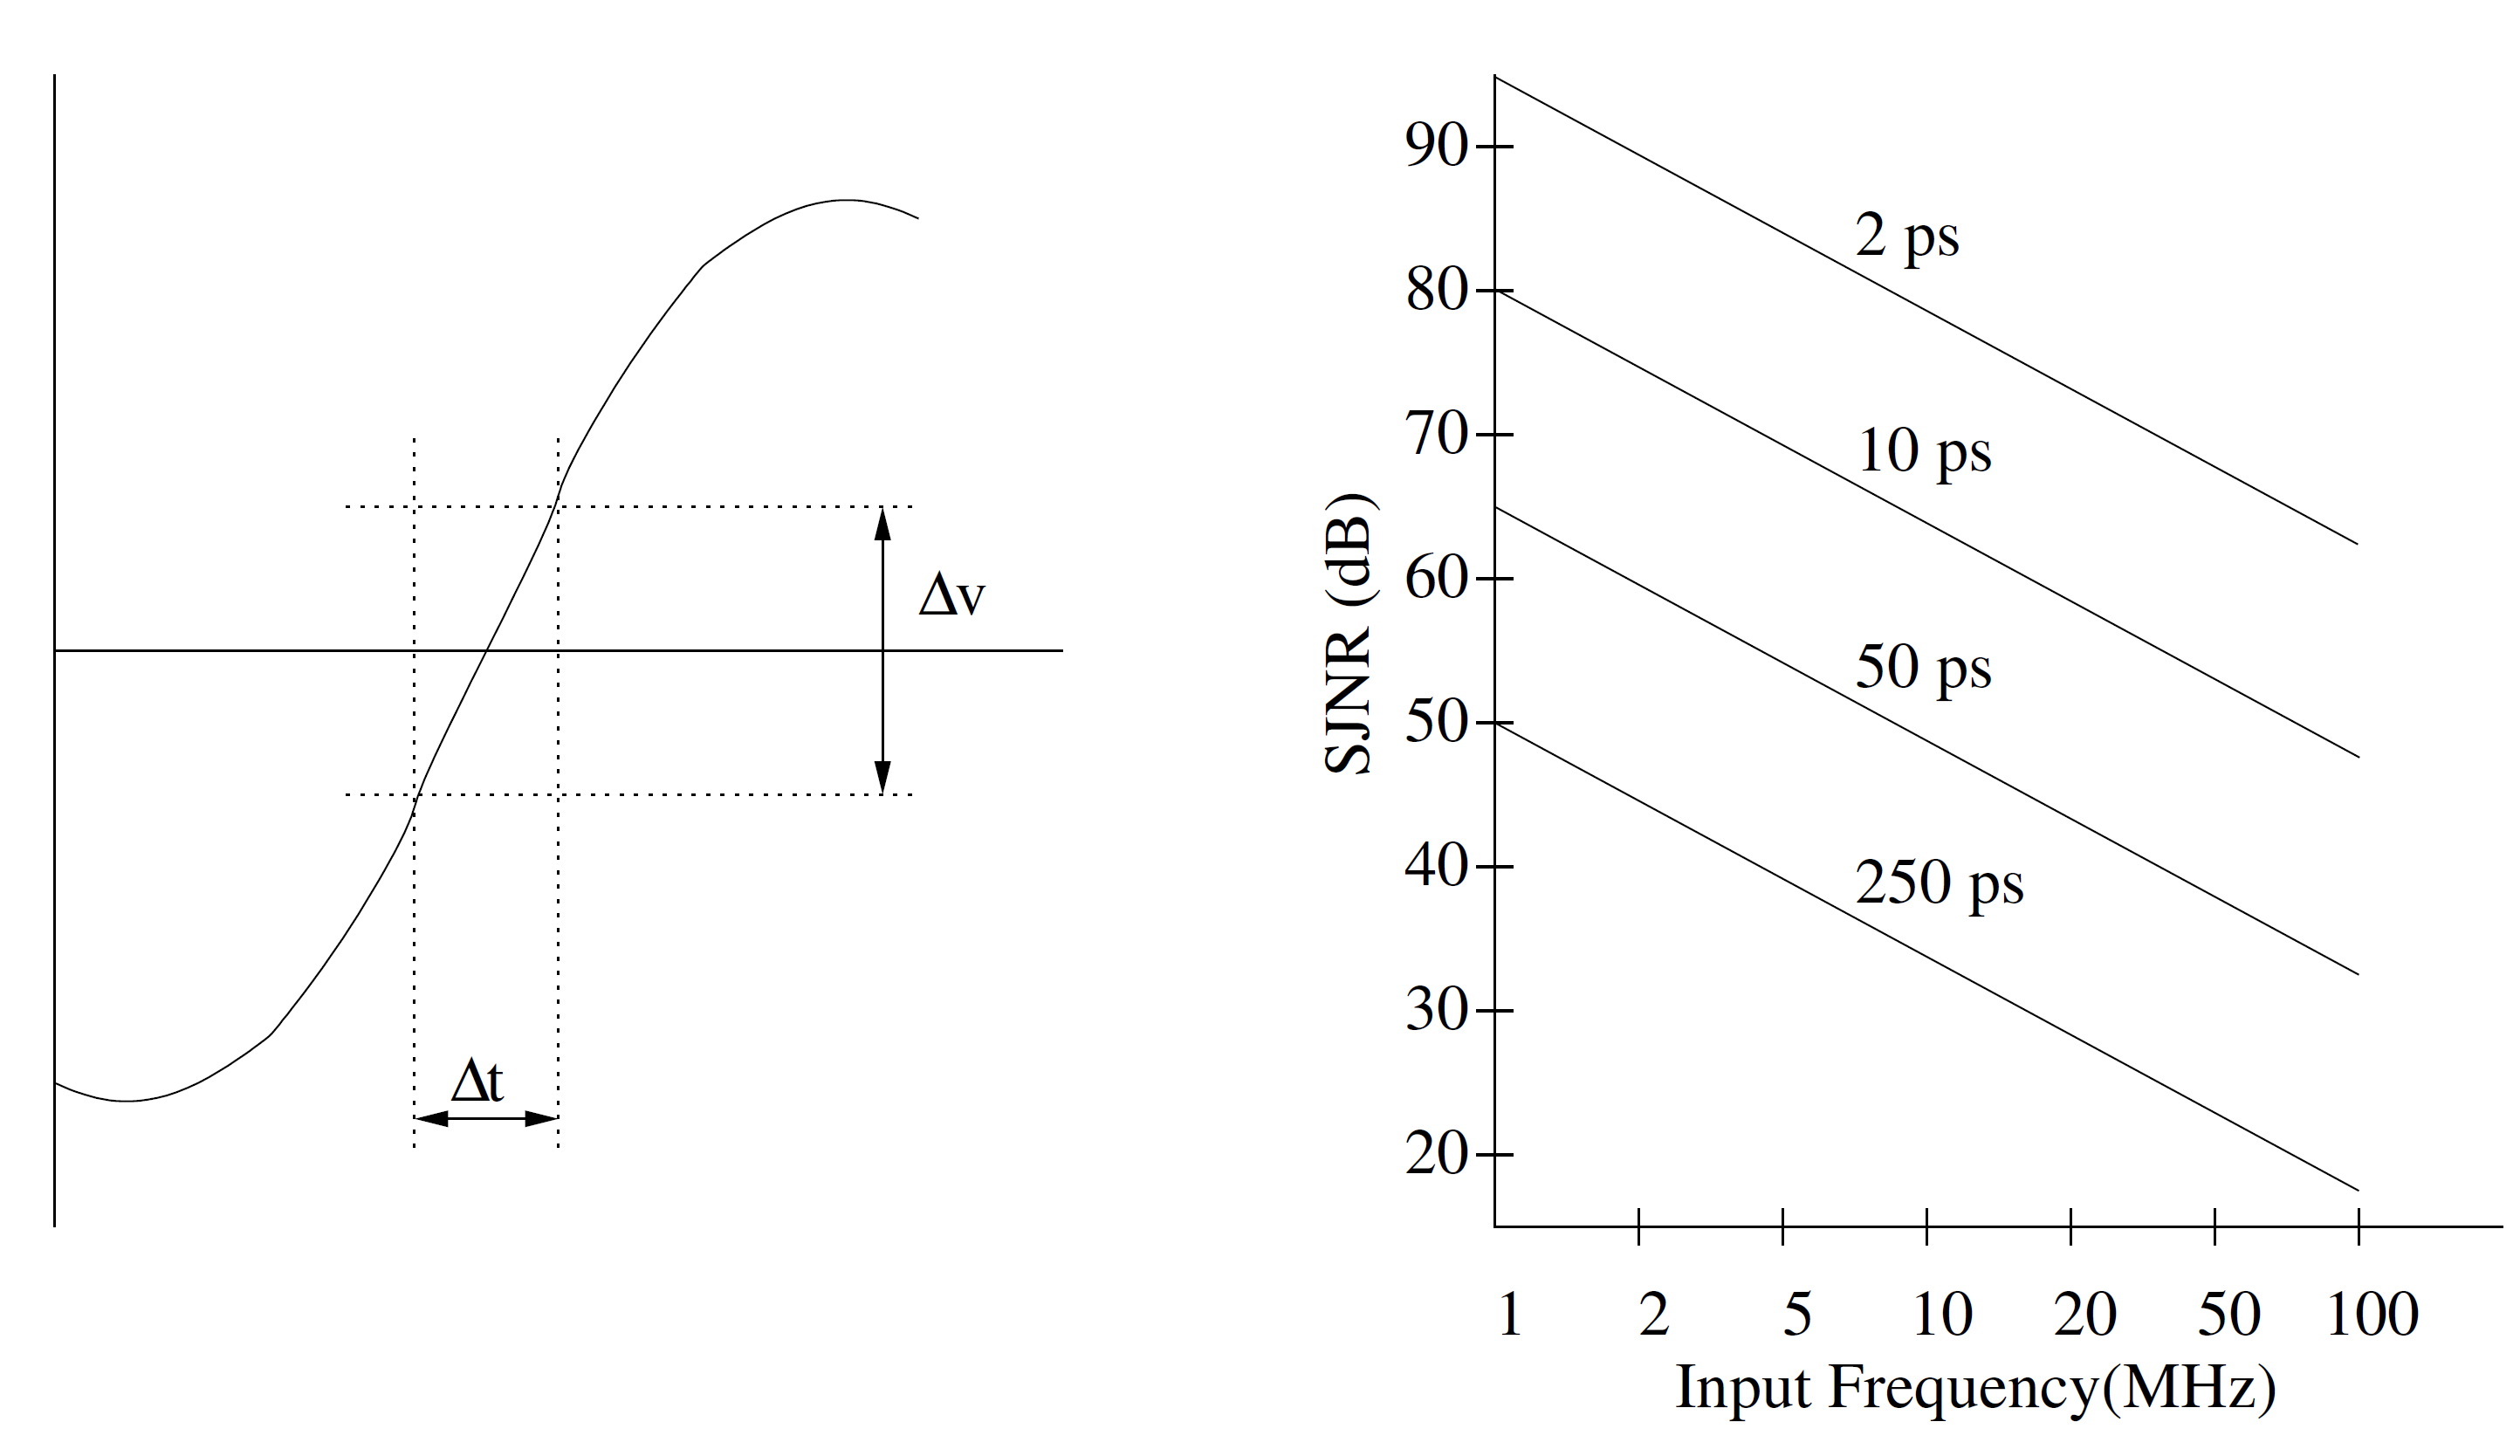
\includegraphics[width = \textwidth]{chap/02-theory/img/ap_jit}
	\caption{Placeholder: Effects of aperture jitter and SJNR \cite{Lundberg}}
	\label{fig:ap_jit}
\end{figure}
%todo to tikz

\paragraph{Transient Response}
The \textit{transient response} denotes the settling time of an \gls{adc} until full accuracy ($\pm$ 1/2 \gls{lsb})



\subsubsection*{Time Interleaving}\label{sssec:time-interleaving}
In the \textit{Time Interleaving} technique multiple \glspl{adc} are used in such way, that allows to sample data at a faster rate, than the respective sample rate of each individual \gls{adc}. The principle is based on time-multiplexing an array of $M$ identical \glspl{adc} (see \autoref{fig:adc_interleaving}), each sampling at $f_c = f_s/M$ individually. This means, the \glspl{adc} are clocked in such a way, that they start their respective conversion cycle shortly one after another. At time $t_0$ the first \gls{adc} starts converting the input signal $V_i(t_0)$, after a time delay $\Delta t_i$ the second starts converting the signal $V_i(t_0 + t_i)$, the third converts $V_i(t_0 + 2t_i)$ and so on. After the $M$-th \gls{adc} has sampled the signal $V_i(t_0 + (M-1)t_i)$, the whole cycle starts anew with the first converter. \cite{mangrob}
\begin{figure}[tbh]
	\centering
	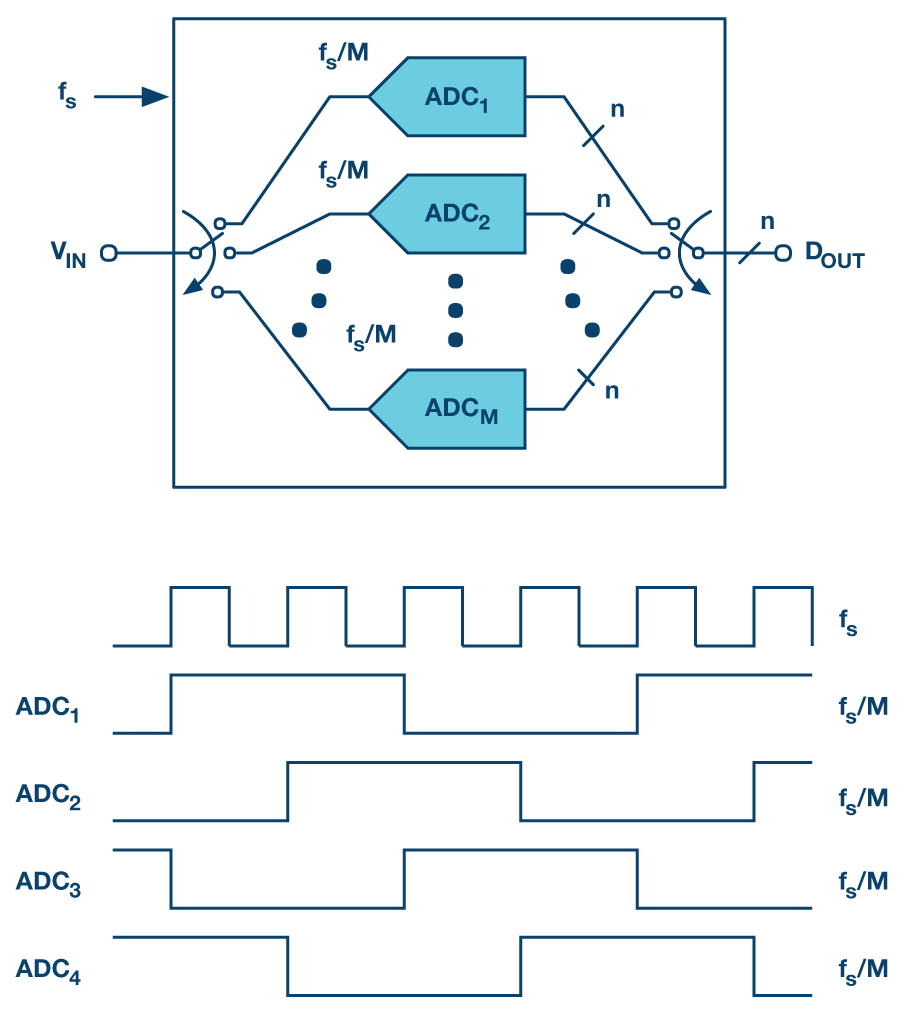
\includegraphics[width = \textwidth]{chap/02-theory/img/adc_inter}
	\caption[Time Interleaving]{Placeholder: An array of $M$ time interleaved $N$-bit \glspl{adc} with example of clocking scheme for the case of $M$ = 4 \cite{mangrob}}
	\label{fig:adc_interleaving}
\end{figure}
%todo to tikz
\paragraph{Challenges}
Spurs appear in the spectrum. There are several reasons for this.

First reason is the \textit{offset mismatch} between den \glspl{adc}. Each \gls{adc} has an DC offset value. Considering as example an interleaving structure with two \glspl{adc} and a constant input voltage: when the samples are acquired back and forth between the two \glspl{adc}, the resulting output will switch back and forth between two levels due to the different offset levels. This output switches at the frequency $f_s/2$ and therefore introduces an additional frequency component in the spectrum (see \autoref{fig:offset_mm}). The magnitude of the spur depends on the offset difference between the \glspl{adc}. \cite{Harris2019}

\begin{figure}[tbh]
	\centering
	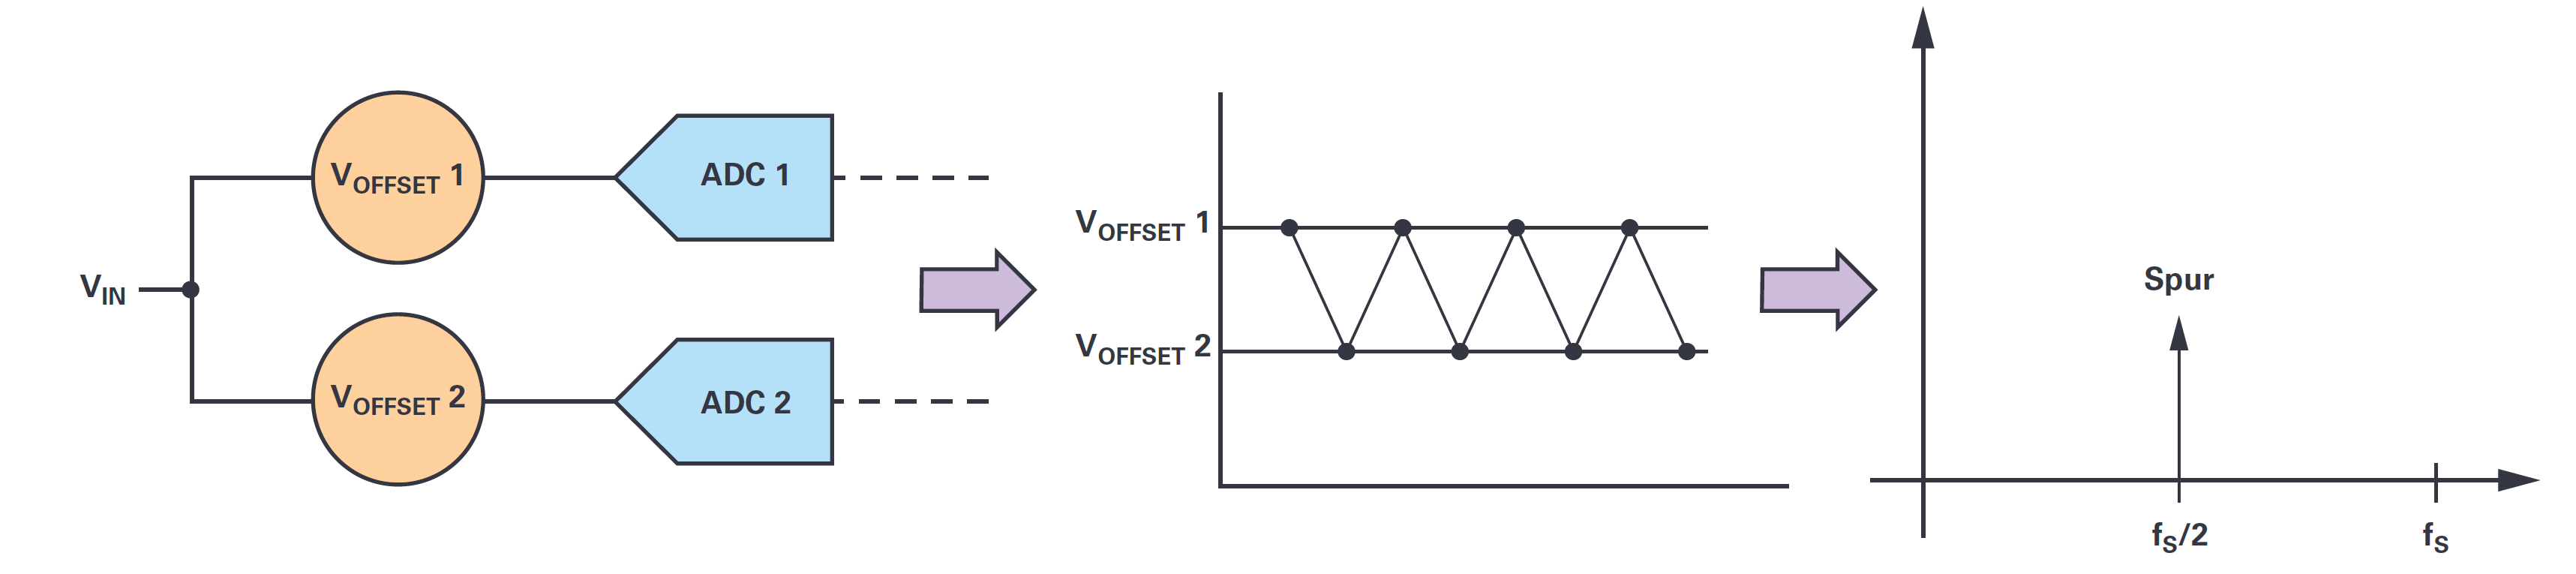
\includegraphics[width = \textwidth]{chap/02-theory/img/offset_mm}
	\caption{Placeholder: Offset-Mismatch in Interleaving \cite{Harris2019}}
	\label{fig:offset_mm}
\end{figure}

Besides of the offset also the gain of the converters can be mismatched. This \textit{gain mismatch} has a frequency component to it, which in case of an input signal of the frequency $f_{\text{in}}$ results in a spur at $f_s/2 \pm f_{\text{in}}$ (see \autoref{fig:gain_mm}). \cite{Harris2019}
\begin{figure}[tbh]
	\centering
	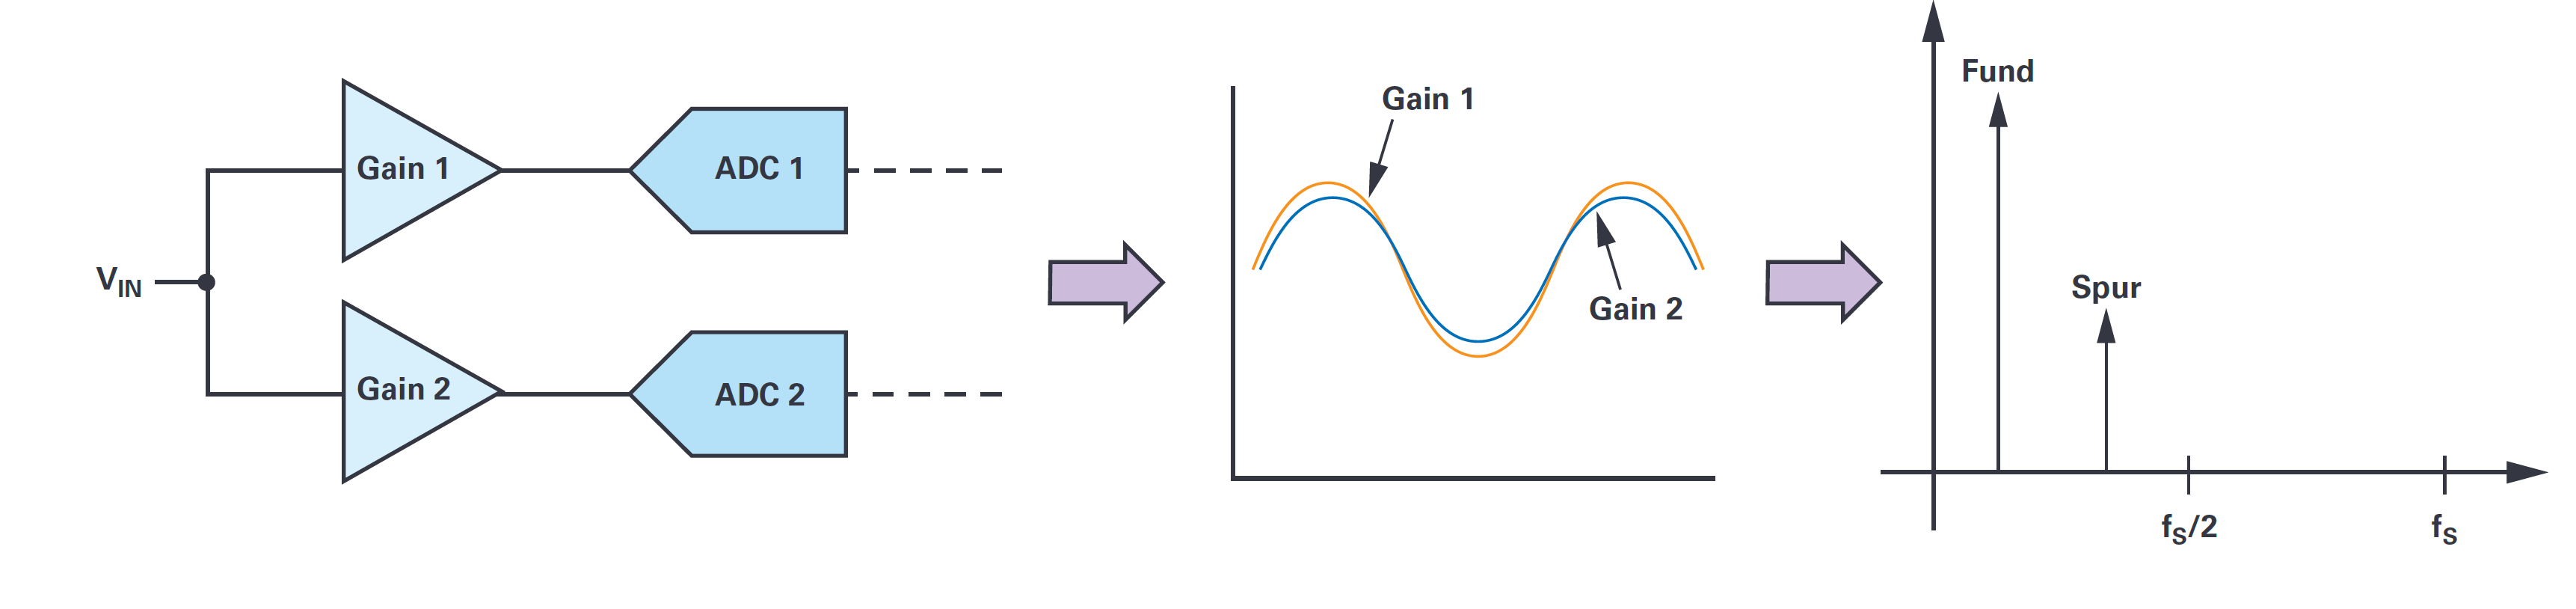
\includegraphics[width = \textwidth]{chap/02-theory/img/gain_mm}
	\caption{Placeholder: Gain-Mismatch in Interleaving \cite{Harris2019}}
	\label{fig:gain_mm}
\end{figure}

In the time domain, \textit{timing mismatch} due to group delay in the analog circuitry of the \gls{adc} and clock skew\footnote{Difference in arrival time of the clock signal at different components.} can occur. The group delay in analog circuitry can vary between the converters. Furthermore, the clock skew has on the one hand an aperture uncertainty component at each of the \glspl{adc} and on the other hand a component related to the accuracy of the clock phases, which are input to each converter. \cite{Harris2019} This mismatch also produces a spur at $f_s/2 \pm f_{\text{in}}$ (see \autoref{fig:timing_mm}).

\begin{figure}[tbh]
	\centering
	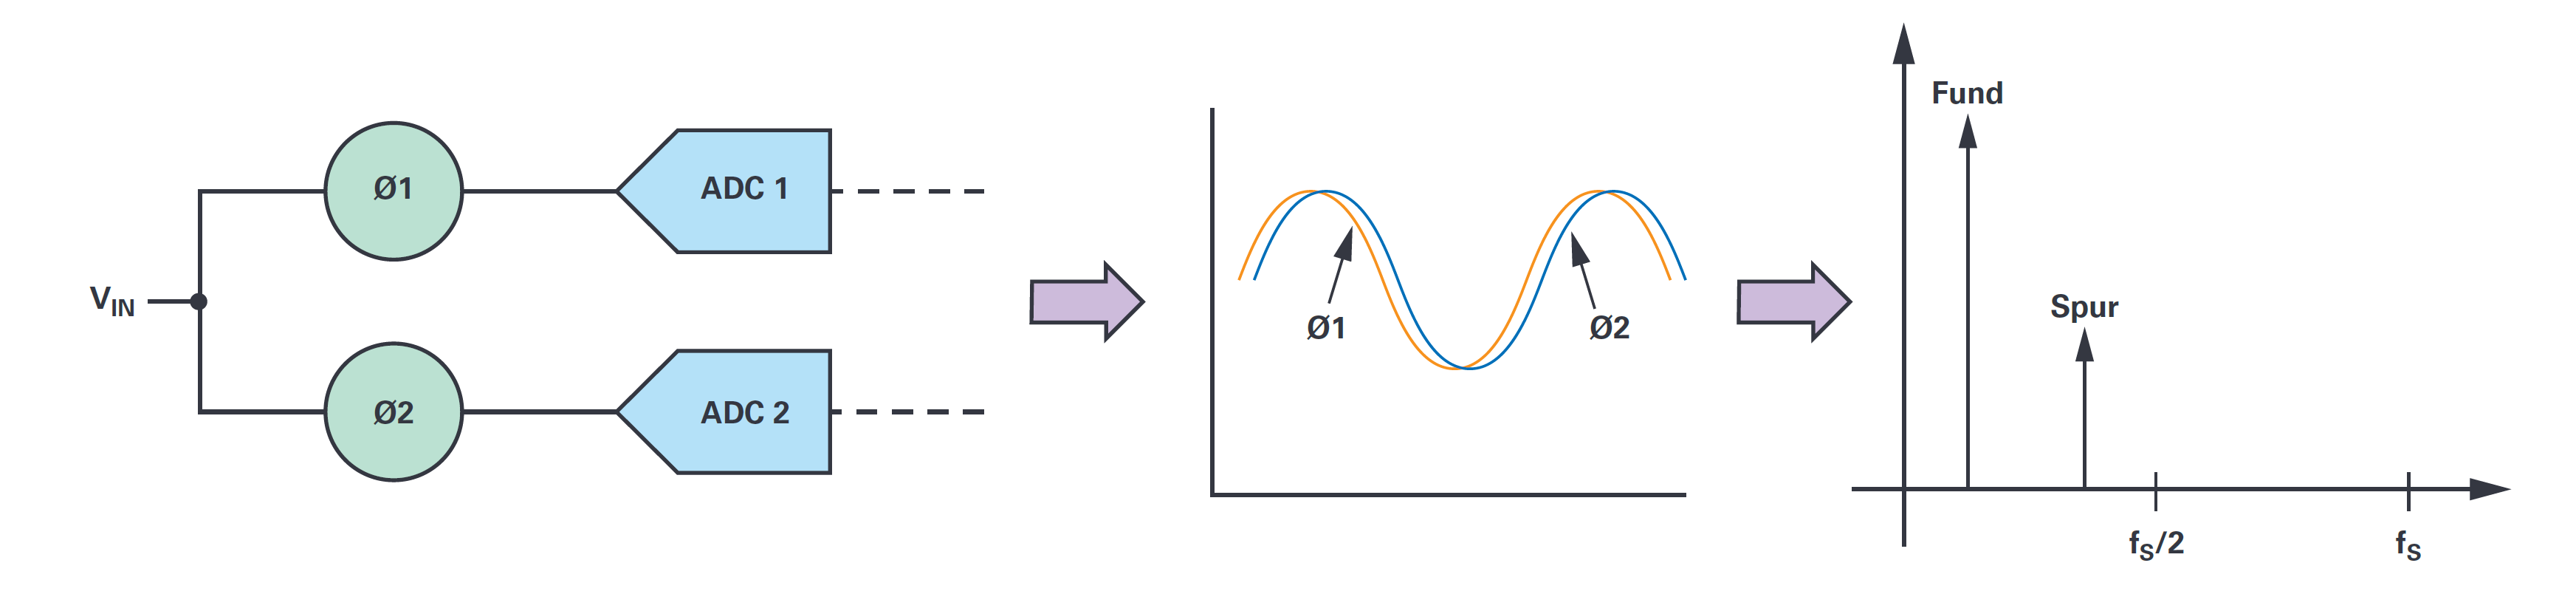
\includegraphics[width = \textwidth]{chap/02-theory/img/timing_mm}
	\caption{Placeholder: Timing-Mismatch in Interleaving \cite{Harris2019}}
	\label{fig:timing_mm}
\end{figure}

The last possible mismatch is the \textit{bandwidth mismatch}, which contains both gain and phase/frequency component (see \autoref{fig:bandwidth_mm}). Due to bandwidth mismatch, different gain values at different frequencies can be seen. An additional timing component causes different delays for signals at different frequencies through each \gls{adc}. Just like gain and timing mismatch, the bandwidth mismatch causes a spur at $f_s/2 \pm f_{\text{in}}$.
\begin{figure}[tbh]
	\centering
	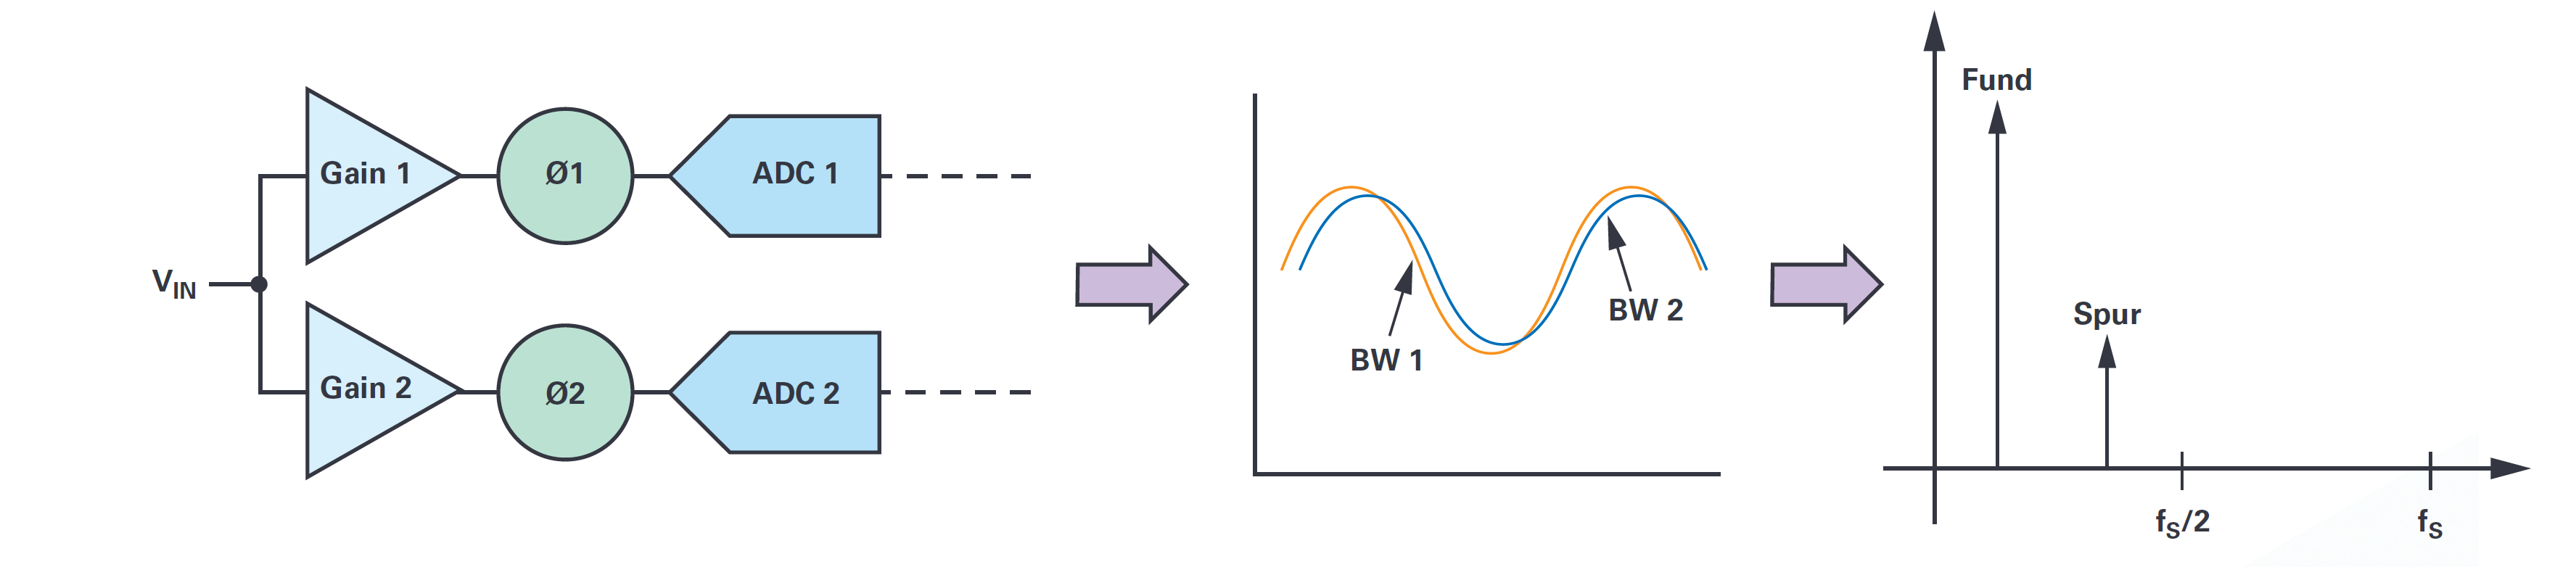
\includegraphics[width = \textwidth]{chap/02-theory/img/bandwidth_mm}
	\caption{Placeholder: Timing-Mismatch in Interleaving \cite{Harris2019}}
	\label{fig:bandwidth_mm}
\end{figure}
